\chapter{Introduction to neural networks}
\section{Theorical Foundation}
\subsection{Supervised dataset}
\paragraph{1. $\bigstar$ What are the train, val and test sets used for?}
The training dataset is utilized to train the model, while the test dataset is employed to assess the model's performance on previously unseen data. Lastly, the validation set constitutes a distinct subset of the dataset employed for the purpose of refining and optimizing the model's hyperparameters.

\paragraph{2. What is the influence of the number of exemples $N$?}
A larger number of examples can enhance the model's capacity to generalize and improve its robustness against noise or outliers. Conversely, a smaller number of examples can make the model susceptible to overfitting. It is important to note that increasing the dataset size can also lead to an escalation in the computational complexity of the model training process.

\subsection{Network architecture}
\paragraph{3. Why is it important to add activation functions between linear transformations?}
Otherwise, we would simply be aggregating linear functions, resulting in a linear output. Activation functions introduce non-linearity to the network, enabling the model to capture and learn more intricate patterns than those achievable through linear transformations alone.

\paragraph{4. $\bigstar$ What are the sizes $n_x$, $n_h$, $n_y$ in the figure 1? In practice, how are these sizes chosen?}
\begin{itemize}
    \item $n_x = 2$ represents the input size (data dimension).
    \item $n_h = 4$ represents the hidden layer size, selected based on the desired complexity of features to be learned in the hidden layer. An excessively large size can result in overfitting.
    \item $n_y = 2$ represents the output size, determined according to the number of classes in $y$.
\end{itemize}

\paragraph{5. What do the vectors $\hat{y}$ and $y$ represent? What is the difference between these two quantities?}
$y \in \{0,1\}$ represents the ground truth, where the values are binary (0 or 1).
$\hat{y} \in [0,1]$ represents a probability-like score assigned to each class by the model. $\hat{y}$ reflects the model's level of confidence in its predictions for each class.

\paragraph{6. Why use a $\text{SoftMax}$ function as the output activation function?}
The reason for employing the SoftMax function is to transform $\tilde{y} \in \mathbb{R}$ into a probability distribution, which is especially useful in multi-class classification problems, as it returns the predicted probability for the $j^\mathrm{th}$ class given a sample $x$, $ P(y=j | x) $. 

\paragraph{7. Write the mathematical equations allowing to perform the \textit{forward} pass of the neural network, i.e. allowing to successively produce $\hat{h}$, $ h $, $ \tilde{y} $, $ \hat{y} $, starting at $x$.}
Let $W_i$ and $b_i$ denote the parameters for layer $i$, $f_i(x) = x W_i ^T + b_i$ represent the linear transformation, and $g_i(x)$ be the activation function for layer $i$.

Let's calculate the weighted sum and activation for the first hidden layer:
\begin{align*}
    \tilde{h} & = f_0(x)         \\
    h         & = g_0(\tilde{h})
\end{align*}

Then, let's proceed to the output layer by computing the weighted sum and activation for the output layer:
\begin{align*}
    \tilde{y} & = f_1(h)         \\
    \hat{y}   & = g_1(\tilde{y})
\end{align*}

These equations describe the sequential steps involved in the forward pass of the neural network, ultimately producing the output $\hat{y}$ based on the input $x$.

\subsection{Loss function}
\paragraph{8. During training, we try to minimize the loss function. For cross entropy and squared error, how must the $ \hat{y}_i $  vary to decrease the global loss function $ \mathcal{L} $?}
Our aim is to minimize the loss function $\mathcal{L}$ to train a model effectively.

For the cross-entropy loss, $\hat{y}_i$ should vary in a way that makes it closer to the true target value $y_i$ for each data point. Specifically, when $y_i = 1$, $\hat{y}_i$ should be pushed towards 1. The closer $\hat{y}_i$ is to 1, the lower the loss. Conversely, when $y_i = 0$, $\hat{y}_i$ should be pushed towards 0. The closer $\hat{y}_i$ is to 0, the lower the loss.

For squared error loss, $\hat{y}_i$ should vary in a way that makes it closer to the true target value $y_i$ for each data point. The goal is to minimize the squared difference between $\hat{y}_i$ and $y_i$. This means that if $\hat{y}_i$ is greater than $y_i$, it should decrease, and if $\hat{y}_i$ is smaller than $y_i$, it should increase.

\paragraph{9. How are these functions better suited to classification or regression tasks?}
Cross-entropy loss is better suited for classification tasks for several reasons:

\begin{itemize}
    \item Cross-entropy loss is based on the negative logarithm of the predicted probability of the true class. This logarithmic nature amplifies errors when the predicted probability deviates from 1 (for the correct class) and from 0 (for incorrect classes), depicted in \Cref{fig:CELoss}. Consequently, it effectively penalizes misclassifications, making it particularly suitable for classification tasks. However, it is imperative that $\hat{y}$ remains within the range $[0, 1]$ for this loss to be effective.
    \item Cross-entropy loss is often used in conjunction with the SoftMax activation function in the output layer of neural networks for multi-class classification. The SoftMax function ensures that the predicted probabilities sum to 1, aligning perfectly with the requirements of the cross-entropy loss.
\end{itemize}

\begin{figure}[H]
    \centering
    \includegraphics*[width=0.6\textwidth]{figs/cross_entropy.png}
    \caption{}
    \label{fig:CELoss}
\end{figure}

On the other hand, Mean Squared Error serves a different role and is better suited for regression tasks:

\begin{itemize}
    \item MSE is ideal when dealing with $(y, \hat{y}) \in \mathbb{R}^2$ (as opposed to the bounded interval $[0, 1]$).
    \item MSE is advantageous due to its convexity, which simplifies optimization. However, it's important to note that it may not always be the best choice for every regression task, especially when dealing with outliers, as it can be sensitive to extreme values.
\end{itemize}

\subsection{Optimization algorithm}
\paragraph{10. What seem to be the advantages and disadvantages of the various variants of gradient descent between the classic, mini-batch stochastic and online stochastic versions? Which one seems the most reasonable to use in the general case?}
Gradient computation becomes computationally expensive as it scales with the number of examples included. However, including more examples enhances gradient exploration with precision and stability, analogous to the exploration-exploitation trade-off in reinforcement learning.

Classic gradient descent offers stability, particularly with convex loss functions, featuring deterministic and reproducible updates. Nonetheless, its stability may lead to getting trapped in local minima when dealing with non-convex loss functions. Additionally, it is computationally intensive, especially for large datasets, as it demands evaluating the gradient with the entire dataset in each iteration.

Mini-Batch Stochastic Gradient Descent (SGD) converges faster compared to classic gradient descent by updating model parameters with small, random data subsets (mini-batches). This stochasticity aids in escaping local minima and exploring the loss landscape more efficiently. However, it may introduce noise and oscillations.

On the other hand, Online Stochastic Gradient Descent offers extremely rapid updates, processing one training example at a time, making it suitable for streaming or large-scale online learning scenarios. However, its highly noisy updates can result in erratic convergence or divergence, necessitating careful learning rate tuning.

For training deep neural networks in the general case, mini-batch stochastic gradient descent is the most reasonable choice. It strikes a balance between the computational efficiency of classic gradient descent and the noise resilience and convergence speed of online SGD.

\paragraph{11. $\bigstar$ What is the influence of the \textit{learning rate} $\eta$  on learning?}
The learning rate plays a crucial role in influencing various aspects of the learning process, including convergence speed, stability, and the quality of the final model.

A higher learning rate typically results in faster convergence because it leads to larger updates in model parameters during each iteration. However, an excessively high learning rate can cause issues such as overshooting, where the optimization process diverges or oscillates around the minimum, preventing successful convergence.

Conversely, a smaller learning rate allows the optimization algorithm to take smaller steps, which can be advantageous for exploring local minima more thoroughly and escaping shallow local minima. Nonetheless, if the learning rate is too small, it may lead to slow convergence or getting stuck in local minima.

To address these challenges, various techniques like learning rate schedulers (gradually reducing the learning rate over time) or adaptive learning rate methods (e.g., Adam) have been developed to automate learning rate adjustments during training. The choice of learning rate may also be influenced by the batch size used in mini-batch stochastic gradient descent, as smaller batch sizes may require smaller learning rates to maintain stability.

In practice, selecting an appropriate learning rate often involves experimentation and can be problem-specific. Techniques such as grid search or random search, in combination with cross-validation, can aid in determining an optimal learning rate for a particular task.

\paragraph{12. $\bigstar$ Compare the complexity (depending on the number of layers in the network) of calculating the gradients of the \textit{loss} with respect to the parameters, using the naive approach and the \textit{backprop} algorithm.}
The naive method involves calculating the gradient of the loss function with respect to each parameter independently. For a network with a large number of parameters, this is computationally expensive and inefficient, essentially repeating a substantial amount of calculation needlessly. The complexity becomes substantial as the number of layers (and, as a result, the number of parameters) increases. It becomes a combinatorial problem with a complexity is $ \mathcal{O}(n!) $ where $n$ is the number of layers.

On the other hand, backpropagation leverages the chain rule from calculus to efficiently calculate gradients, making it a much more efficient strategy. It breaks down the complex task of computing derivatives for a multi-stage function into smaller, more manageable steps. This approach significantly reduces the computational burden, especially for networks with a large number of interconnected layers and parameters. Its complexity is linear, $\mathcal{O}(n)$, making it a much more practical choice for training deep neural networks.

\paragraph{13. What criteria must the network architecture meet to allow such an optimization procedure?}
For the backpropagation algorithm to be applicable, several criteria must be met. First of all, each layer function, including the activation functions and the loss function, must be differentiable with respect to their parameters. This is crucial for calculating gradients during the training process. Furthermore, as backpropagation relies on the sequential flow of information from the input layer to the output layer, the network architecture should possess a feedforward, sequential structure without loops or recurrent connections. Loops or recurrent connections can introduce complications in gradient calculations.

\paragraph{14. The function SoftMax and the \textit{loss} of \textit{cross-entropy} are often used together and their gradient is very simple. Show that the \textit{loss} can be simplified by:
    \[l = - \sum_{i}^{} y_i \tilde{y}_i + \log_{} \left(\sum_{i}^{} e^{\tilde{y}_i}\right)\]}
Let us define the cross-entropy loss as \( l(y, \hat{y}) = - \sum_{i=1}^{n_y} y_i \log \hat{y}_i \), where \( n_y \) represents the total number of classes. The SoftMax function for a vector \( \tilde{y} \in \mathbb{R}^D \) is defined as \( \text{SoftMax}(\tilde{y_i}) = \frac{e^{\tilde{y_i}}}{\sum_{j=1}^{n_y} e^{\tilde{y_j}}} \). Notably, the output of the SoftMax function serves as the input for the cross-entropy loss, denoted as \( \hat{y}_i = \text{SoftMax}(\tilde{y_i}) \). Let us substitute this value into the expression.

\begin{align*}
    l(y, \hat{y}) & = - \sum_{i=1}^{n_y} y_i \log_{} \hat{y}_i                                                                 \\
                  & = - \sum_{i=1}^{n_y} y_i \log_{} \text{SoftMax}(\tilde{y_i})                                               \\
                  & = - \sum_{i=1}^{n_y} y_i \log_{} \frac{e^{\tilde{y_i}}}{\sum_{j=1}^{n_y} e^{\tilde{y_j}} }                   \\
                  & = - \sum_{i=1}^{n_y} y_i \left[ \log_{} e^{\tilde{y}_i} - \log_{} \sum_{j=1}^{n_y} e^{\tilde{y}_j}  \right]  \\
                  & = - \sum_{i=1}^{n_y} y_i \tilde{y}_i - y_i \log_{} \left( \sum_{j=1}^{n_y}e^{\tilde{y}_j} \right)                           \\
                  & = - \sum_{i=1}^{n_y} y_i \tilde{y}_i + \sum_{i=1}^{n_y} y_i \log_{} \left(\sum_{j}^{n_y}e^{\tilde{y}_j}\right) \\
                  & = - \sum_{i=1}^{n_y} y_i \tilde{y}_i + \log_{} \left(\sum_{j}^{n_y}e^{\tilde{y}_j}\right) \sum_{i=1}^{n_y} y_i
\end{align*}

Since $y_i$ is one-hot encoded, we know that $\sum_{i=1}^{n_y} y_i = 1$. Thus, we have the final expression for the cross-entropy loss:

\[ l(y, \hat{y}) = - \sum_{i=1}^{n_y} y_i \tilde{y}_i + \log_{} \left(\sum_{i=1}^{n_y} e^{\tilde{y}_i}\right) \]

\paragraph{15. Write the gradient of the \textit{loss} (\textit{cross-entropy}) relative to the intermediate output $ \tilde{y} $ }
\begin{align*}
    \frac{\partial l}{\partial \tilde{y}_i} & = -y_i + \frac{\frac{\partial }{\partial \tilde{y}_i } (\sum_{j=1}^{n_y} e^{ \tilde{y}_j })}{\sum_{j=1}^{n_y} e^{ \tilde{y}_j }} \\
                                            & = - y_i + \frac{e^{\tilde{y}_i}}{\sum_{j=1}^{n_y} e^{ \tilde{y}_j}}                                                          \\
                                            & = - y_i + \text{SoftMax}(\tilde{y})_i
\end{align*}
\[
    \nabla _{\tilde{y}}l = \begin{pmatrix}
        \frac{\partial l}{\partial \tilde{y}_1} \\
        \vdots                                  \\
        \frac{\partial l}{\partial \tilde{y}_{n_y}}
    \end{pmatrix} = \begin{pmatrix}
        \text{SoftMax}(\tilde{y})_1 - y_1 \\
        \vdots                            \\
        \text{SoftMax}(\tilde{y})_{n_y} - y_{n_y}
    \end{pmatrix} \\
    = \hat{y} - y
\]

\paragraph{16. Using the \textit{backpropagation}, write the gradient of the \textit{loss} with respect to the weights of the output layer $ \nabla _{W_y}l $ . Note that writing this gradient uses $ \nabla _{\tilde{y}}l $ . Do the same for $ \nabla _{b_y}l $.\\}

Starting with \( \nabla _{W_y} l \), we have:

\[
    \frac{\partial l}{\partial W_{y,ij}} = \sum_{k}^{} \frac{\partial l}{\partial \tilde{y}_k} \frac{\partial \tilde{y}_k}{\partial W_{y,ij}}
\]

This can be expressed as a matrix:

\[
    \nabla_{W_y} l = \begin{pmatrix}
        \frac{\partial l}{\partial W_{y, 1,1}}   & \dots  & \frac{\partial l}{\partial W_{y, 1,n_h}}    \\
        \vdots                                   & \ddots & \vdots                                      \\
        \frac{\partial l}{\partial W_{y, n_y,1}} & \dots  & \frac{\partial l}{\partial W_{y, n_y, n_h}}
    \end{pmatrix}
\]

First, let's compute $ \tilde{y}_k $
\begin{align*}
    \tilde{y}   & = h W_y^T + b^y                                                                                                        \\
                & = \begin{pmatrix}
        h_{1} & \dots & h_{n_h}
    \end{pmatrix} * \begin{pmatrix}
        W_{1, 1}   & \dots  & W_{1, n_y}   \\
        \vdots     & \ddots & \vdots       \\
        W_{n_h, 1} & \dots  & W_{n_h, n_y} \\
    \end{pmatrix} + \begin{pmatrix}
        b^y_1 & \dots & b^y_{n_y}
    \end{pmatrix}                                 \\
                & = \begin{pmatrix}
        \sum_{j=1}^{n_h} W^y_{1,j} h_{j} + b^y_1 & \sum_{j=1}^{n_h} W^y_{2,j} h_{j} + b^y_2 & \dots & \sum_{j=1}^{n_h} W^y_{n_h,j} h_{k,j} + b^y_{n_h}
    \end{pmatrix}                                                           & \in \mathbb{R}^{1 \times n_h} \\
    \tilde{y}_k & = \sum_{j=1}^{n_h} W^y_{k,j} h_{j} + b_k^y, k \in [1, n_h]
\end{align*}

With this expression, we can now proceed with the calculation of the partial derivative of \( \tilde{y}_k \) with respect to \( W^y_{ij} \):

\[
    \frac{\partial \tilde{y}_k }{\partial W^y_{ij}} = \begin{cases}
        h_j & \text{ if } i=k   \\
        0   & \text{ otherwise}
    \end{cases}
\]

Now, we need to find \( \frac{\partial l}{\partial \tilde{y}_k} \). From the previous question, we have:

\[
    \frac{\partial l}{\partial \tilde{y}_k} = -y_k + \text{SoftMax}(\tilde{y})_k = \hat{y}_k - y_k
\]

Now, combining these results:

\[
    \frac{\partial l}{\partial W_{i,j}^y} = \sum_{k=1}^{n_h} \frac{\partial l}{\partial \tilde{y}_k} \frac{\partial \tilde{y}_k}{\partial W_{i,j}^y} =  \frac{\partial l}{\partial \tilde{y}_i} \frac{\partial \tilde{y}_i}{\partial W_{i,j}^y} = (\hat{y}_i - y_i) h_j = (\nabla _{W_y} l)_{i,j}
\]

So, the gradient of the loss with respect to the weights of the output layer \( \nabla_{W_y} l \) is given by \( \nabla _{\tilde{y}} ^T h \).

\begin{align*}
    \nabla_{W_y} l & = \begin{pmatrix}
        \frac{\partial l}{\partial W^y_{1,1}}   & \dots  & \frac{\partial l}{\partial W^y_{1,n_h}}    \\
        \vdots                                  & \ddots & \vdots                                     \\
        \frac{\partial l}{\partial W^y_{n_y,1}} & \dots  & \frac{\partial l}{\partial W^y_{n_y, n_h}}
    \end{pmatrix}                            \\
                   & = \begin{pmatrix}
        (\hat{y}_1 - y_1) h_{1}         & \dots  & (\hat{y}_1 - y_1) h_{n_h}         \\
        \vdots                          & \ddots & \vdots                            \\
        (\hat{y}_{n_y} - y_{n_y}) h_{1} & \dots  & (\hat{y}_{n_y} - y_{n_y}) h_{n_h}
    \end{pmatrix}                            \\
                   & = \begin{pmatrix}
        \hat{y}_1 - y_1 \\
        \vdots          \\
        \hat{y}_{n_y} - y_{n_y}
    \end{pmatrix} \begin{pmatrix}
        h_1 & h_2 & \dots & h_{n_h}
    \end{pmatrix} \\
                   & = \nabla _{\tilde{y}} ^T h
\end{align*}


% For the gradient with respect to the biases of the output layer \( \nabla_{b_y} l \), the calculation would be similar but would involve the derivative of \( \tilde{y}_k \) with respect to \( b_k^y \), which would be 1, and the gradient \( \frac{\partial l}{\partial \tilde{y}_k} \) remains the same. Putting it all together:

% \[
% \frac{\partial l}{\partial b_k^y} = \sum_{k=1}^{n_h} \frac{\partial l}{\partial \tilde{y}_k} \frac{\partial \tilde{y}_k}{\partial b_k^y} = (\hat{y}_k - y_k) \cdot 1 = \hat{y}_k - y_k
% \]

\paragraph{17. $\bigstar$ Compute other gradients : $ \nabla _{\tilde{h}} l, \nabla _{W_h} l, \nabla_{b_h}l $ }

\begin{enumerate}
    \item The gradient of the loss with respect to \( \tilde{h} \) can be computed using the chain rule:
          \[
              \frac{\partial l}{\partial \tilde{h}_i} = \sum_{k}^{} \frac{\partial l}{\partial h_k} \frac{\partial h_k}{\partial \tilde{h}_i}
          \]
          Let's compute those two terms:
          \[
              \frac{\partial h_k}{\partial \tilde{h}_i} = \frac{\partial \tanh (\tilde{h_k})}{\partial \tilde{h_i}} = \begin{cases}
                  1 - \tanh^2 (\tilde{h_i}) = 1 - h_i^2 & \text{ if } k = i \\
                  0                                     & \text{ otherwise} \\
              \end{cases}
          \]

          Having $ \tilde{y}_i = \sum_{j=1}^{n_h} W_{i,j}^y h_j +b_i^y$ in mind and recovering $ \frac{\partial l}{\partial \tilde{y}_i} = \hat{y}_i - y_i = \delta ^y_i $ from past question:
          \[
              \frac{\partial l}{\partial h_k} = \sum_{j=1}^{} \frac{\partial l}{\partial \tilde{y_j}} \frac{\partial \tilde{y}_j}{\partial h_k} = \sum_{j=1}^{} \delta ^y_j W^y_{j,k}
          \]

          Finally,
          \begin{align*}
              \frac{\partial l}{\partial \tilde{h}_i} & = \sum_{k}^{} \frac{\partial l}{\partial h_k} \frac{\partial h_k}{\partial \tilde{h}_i} \\
                                                      & = \sum_{k}^{} \sum_{j}^{} \delta ^y_j W^y_{j,k} \times \begin{cases}
                  1 - h_i^2 & \text{ if } k = i \\
                  0         & \text{ otherwise} \\
              \end{cases}       \\
                                                      & = (1 - h_i^2) \left(\sum_{j}^{} \delta ^y_j W^y_{j,i}\right)                            \\
                                                      & = \delta ^h _i
          \end{align*}
          So, the gradient \( \nabla _{\tilde{h}} l \) is a vector with elements $ \delta ^h _i $:

          \[
              \nabla _{\tilde{h}} l = (1 - h^2) \odot (\nabla _{\tilde{y}} l * W^y)
          \]


    \item $ \nabla _{W^h} l $ is a matrix composed of elements
          \[
              \frac{\partial l}{\partial W^h _{i,j}} = \sum_{k}^{} \frac{\partial l}{\partial \tilde{h}_k} \frac{\partial \tilde{h}_k}{\partial W^h_{i,j}}
          \]
          From the previous question, we already have $ \frac{\partial l}{\partial h_k} = (1 - h_k^2) (\sum_{j}^{} \delta ^y_j W^y_{j,k}) = \delta_k^h$. So let's compute the other term $ \frac{\partial \tilde{h}_k}{\partial W^h_{i,j}}  $ from $ \tilde{h}_k = \sum_{j=1}^{n_x} W^h_{k,j} x_j + b_k^h $

          \[
              \frac{\partial \tilde{h}_k}{\partial W^h_{i,j}} = \begin{cases}
                  x_j & \text{ if } k = i  \\
                  0   & \text{ otherwise } \\
              \end{cases}
          \]
          So:
          \begin{align*}
              \frac{\partial l}{\partial W^h _{i,j}} & = \sum_{k}^{} \frac{\partial l}{\partial \tilde{h}_k} \frac{\partial \tilde{h}_k}{\partial W^h_{i,j}} \\
                                                     & = \sum_{k}^{}\delta ^h_k \times \begin{cases}
                  x_j & \text{ if } k = i  \\
                  0   & \text{ otherwise } \\
              \end{cases}                                            \\
                                                     & = \delta _i^h x_j                                                                                     \\
              \nabla _W^h                            & = \nabla _{\tilde{h}} ^T l * x
          \end{align*}


    \item Last but not least:
          \[
              \frac{\partial l}{\partial b_i^j} = \sum_{k}^{} \frac{\partial l}{\partial \tilde{h}_k} \frac{\partial \tilde{h}_k}{\partial b_i^h} = \sum_{k}^{}\delta _k^h * \begin{cases}
                  1 & \text{ if } k = i \\
                  0 & \text{ else}      \\
              \end{cases} = \delta ^h_i
          \]

          \[
              \nabla _{b^h} = \nabla _{\tilde{h}} l
          \]

\end{enumerate}

\section{Implementation}

In this section, the primary focus was on exploring how a simple neural network model can perform at classifying tasks which can be difficult with normal machine learning techniques. The context varied from circular data to image classification, and the overall approach was to confirm the theory of precedent section and experiment with different hyperparameters to understand their effects on model performance.

\subsection{Forward and backward manuals}
In neural network training using SGD, it is common practice to average the gradients calculated during the backward pass over the batch size. The idea behind this scaling is to make the learning rate independent of the batch size, so that the updates to the model parameters are roughly consistent regardless of the batch size. We compared these two approaches in \Cref{fig:manual_nn}.

One significant observation is that when using batch averaging, the network requires much more time to achieve its performance, needing 100 epochs instead of 10. However, the trade-off is that the training process becomes much more stable.

\begin{figure}[H]
    \centering
    \begin{subfigure}{0.45\textwidth}
        \centering
        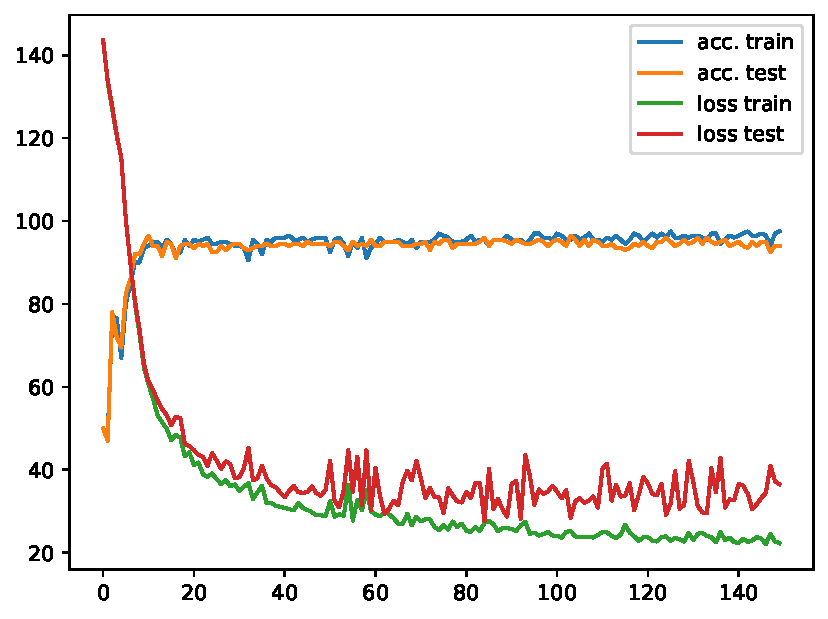
\includegraphics[width=\textwidth]{figs/NN/manual_acc_loss.pdf}
        \caption{Accuracy and losses curves without batch size averaging}
        \label{subfig:manual_acc_loss}
    \end{subfigure}
    \begin{subfigure}{0.45\textwidth}
        \centering
        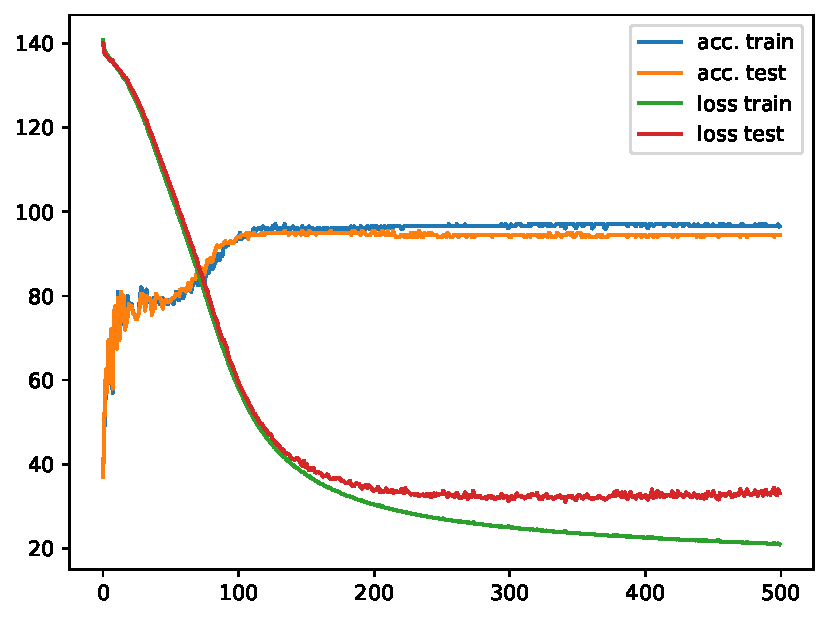
\includegraphics[width=\textwidth]{figs/NN/manual_acc_loss_bis.pdf}
        \caption{Accuracy and losses curves with batch size averaging}
        \label{subfig:manual_acc_loss_bis}
    \end{subfigure}
    \caption{To batch average, or not to batch average.}
    \label{fig:manual_nn}
\end{figure}

In the following experiments, we have chosen to continue with batch averaging. We then proceeded to investigate the influence of learning rate and batch size. The results are presented in \Cref{fig:manual_bs_lr}. Our findings align with the expectations discussed in Question 11.

\begin{figure}[H]
    \centering
    \begin{subfigure}{0.45\textwidth}
        \centering
        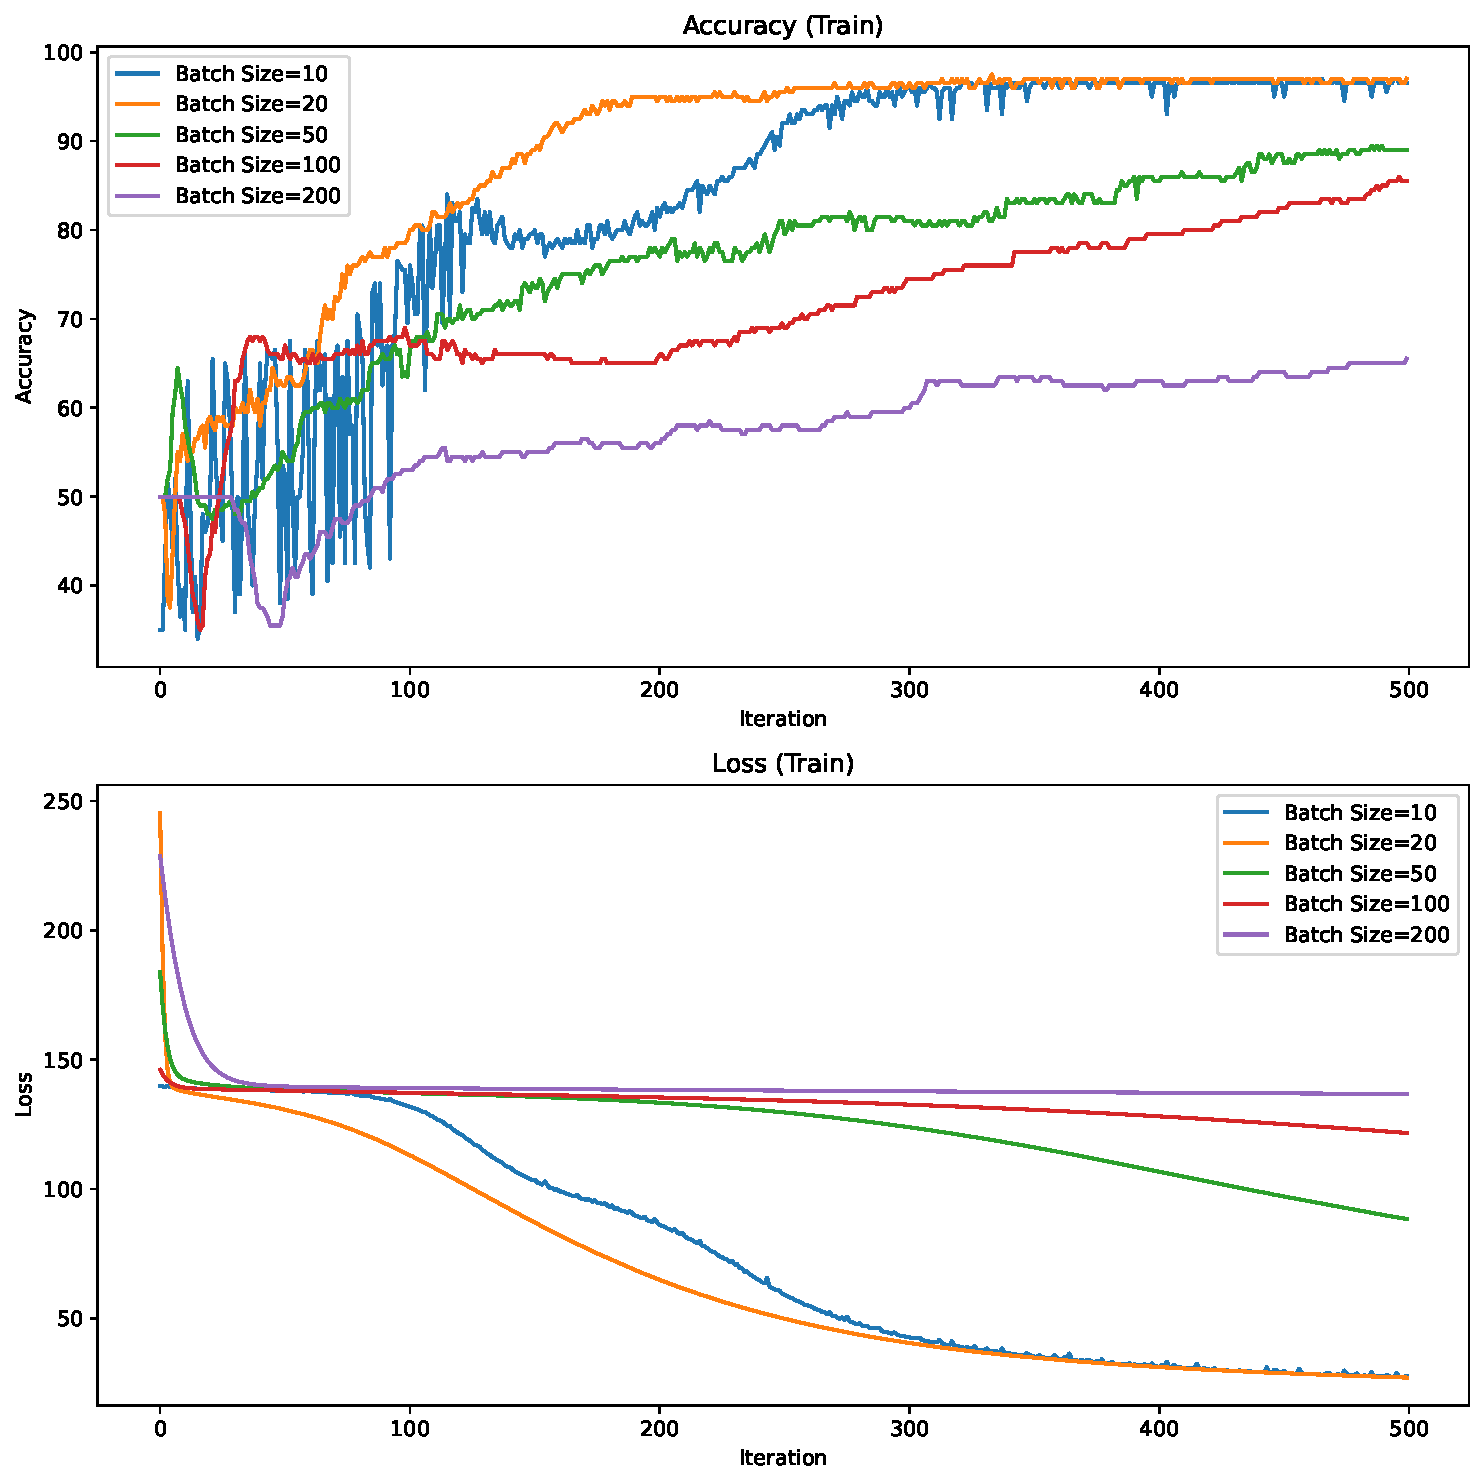
\includegraphics[width=\textwidth]{figs/NN/manual_batchsize.pdf}
        \caption{Influence of batch size}
        \label{subfig:manual_batchsize}
    \end{subfigure}
    \begin{subfigure}{0.45\textwidth}
        \centering
        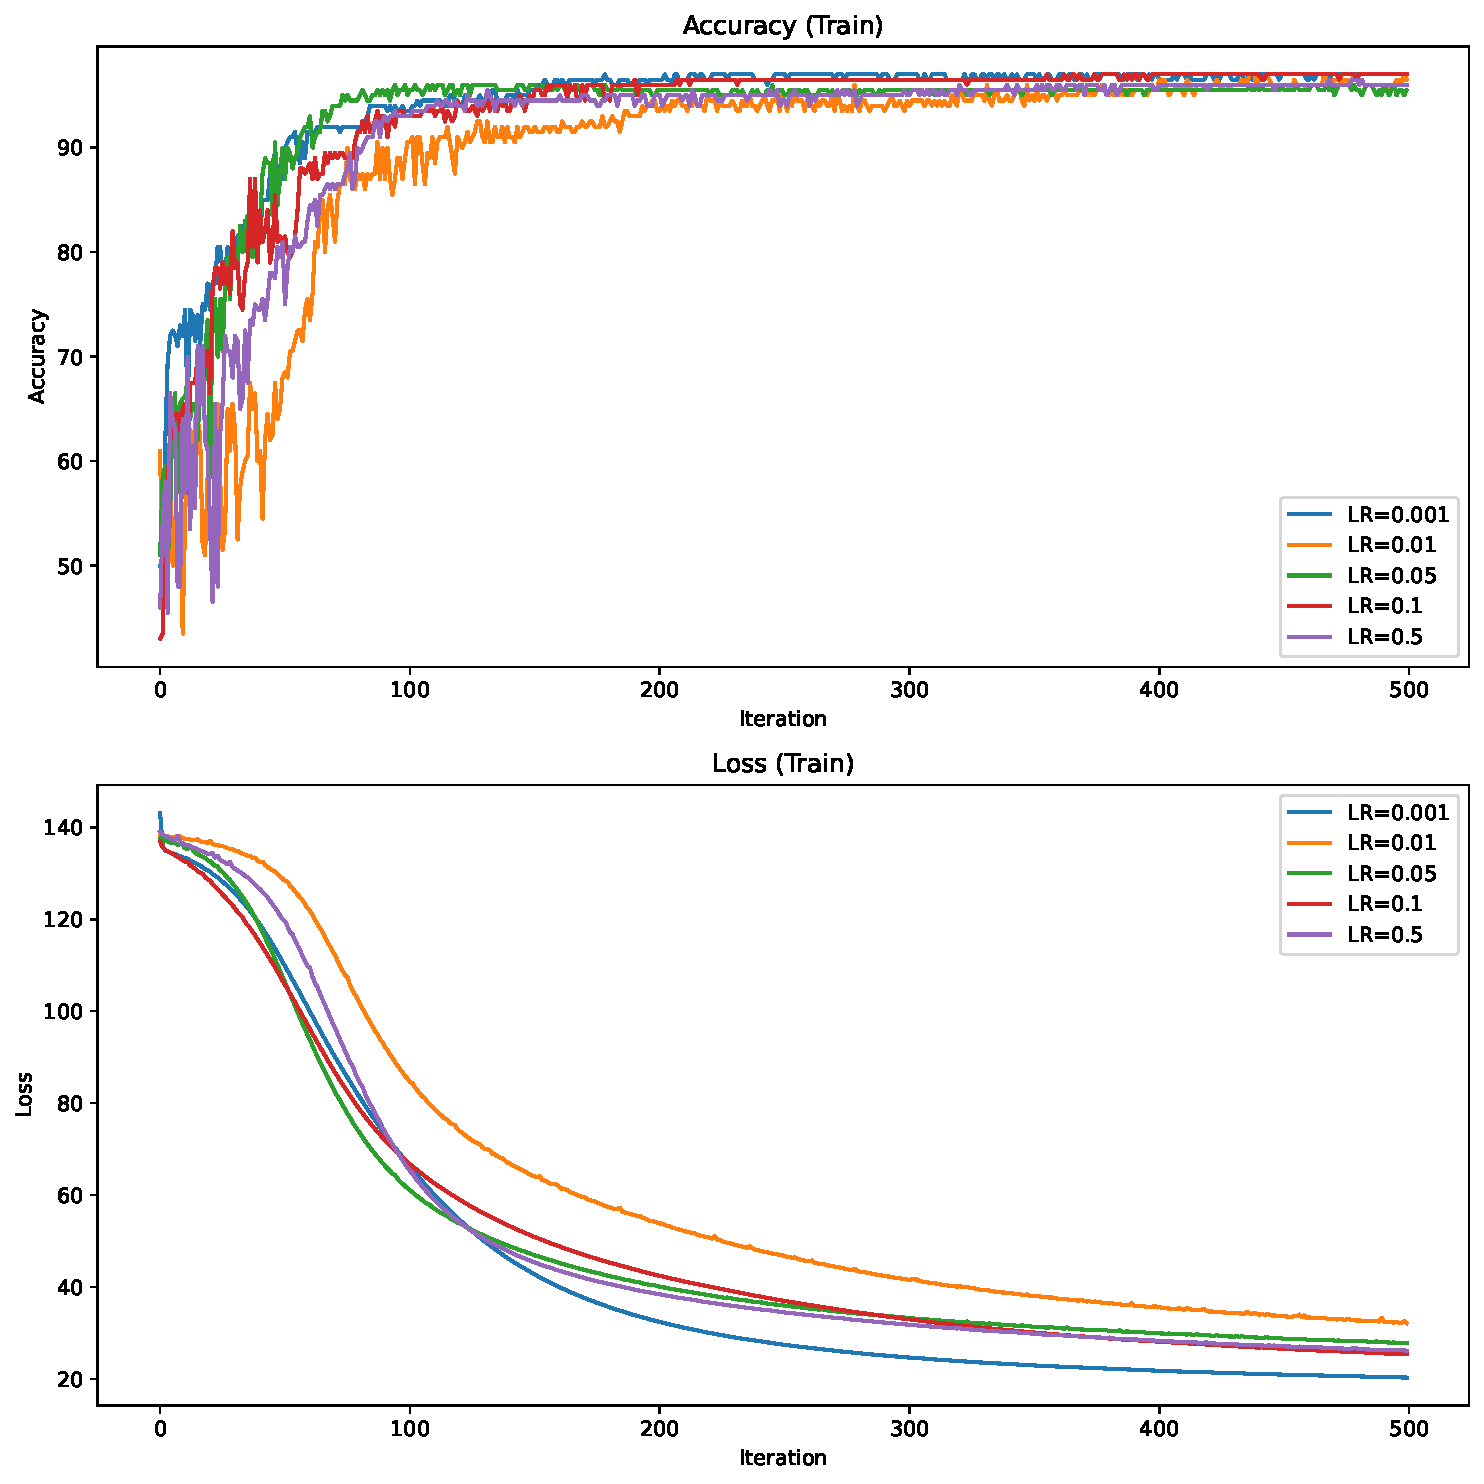
\includegraphics[width=\textwidth]{figs/NN/manual_lr.pdf}
        \caption{Influence of learning rate}
        \label{subfig:manual_lr}
    \end{subfigure}
    \caption{Influence of learning rate and batch size}
    \label{fig:manual_bs_lr}
\end{figure}

In the provided notebook, you will also find animated figures that showcase the evolution of the learning process and the visualization of the decision boundaries. Unexpectedly, by the end of the training, we can observe circular decision boundaries for the circular data as the model is able to classify the data correctly.

% \pagebreak
\subsection{Simplification of the backward pass with \texttt{torch.autograd}}

The results of this section are presented in \Cref{fig:autograd}. It's worth noting that we obtained similar results to when we did not use batch normalization, as indicated by the learning instability. However, our overall conclusions remain consistent.


\begin{figure}[H]
    \centering
    \begin{subfigure}{\textwidth}
        \centering
        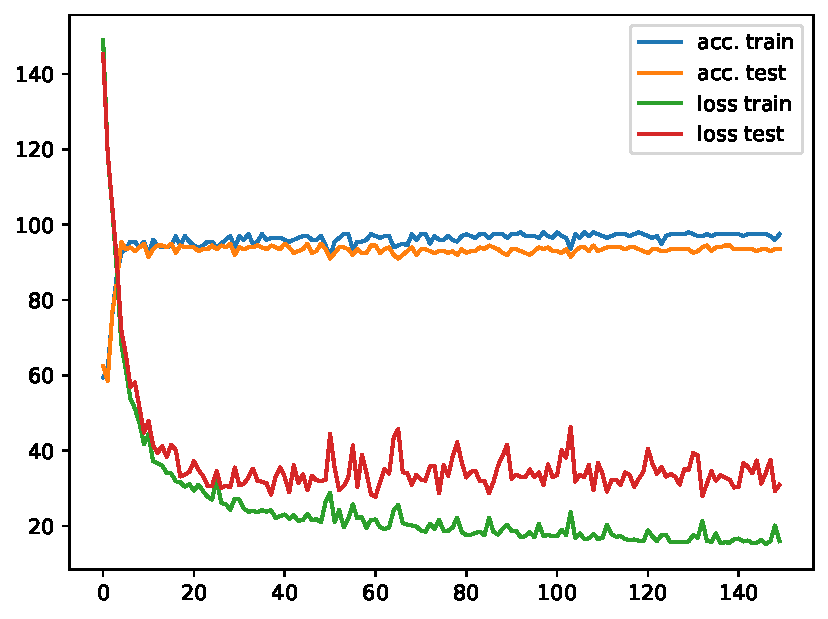
\includegraphics[width=0.5\textwidth, height=5cm]{figs/NN/autograd_acc_loss.pdf}
        \caption{Accuracy and losses curves with \texttt{torch.autograd}}
        \label{subfig:autograd_acc_loss}
    \end{subfigure}
\end{figure}

\begin{figure}[H]\ContinuedFloat
    \centering
    \begin{subfigure}{0.45\textwidth}
        \centering
        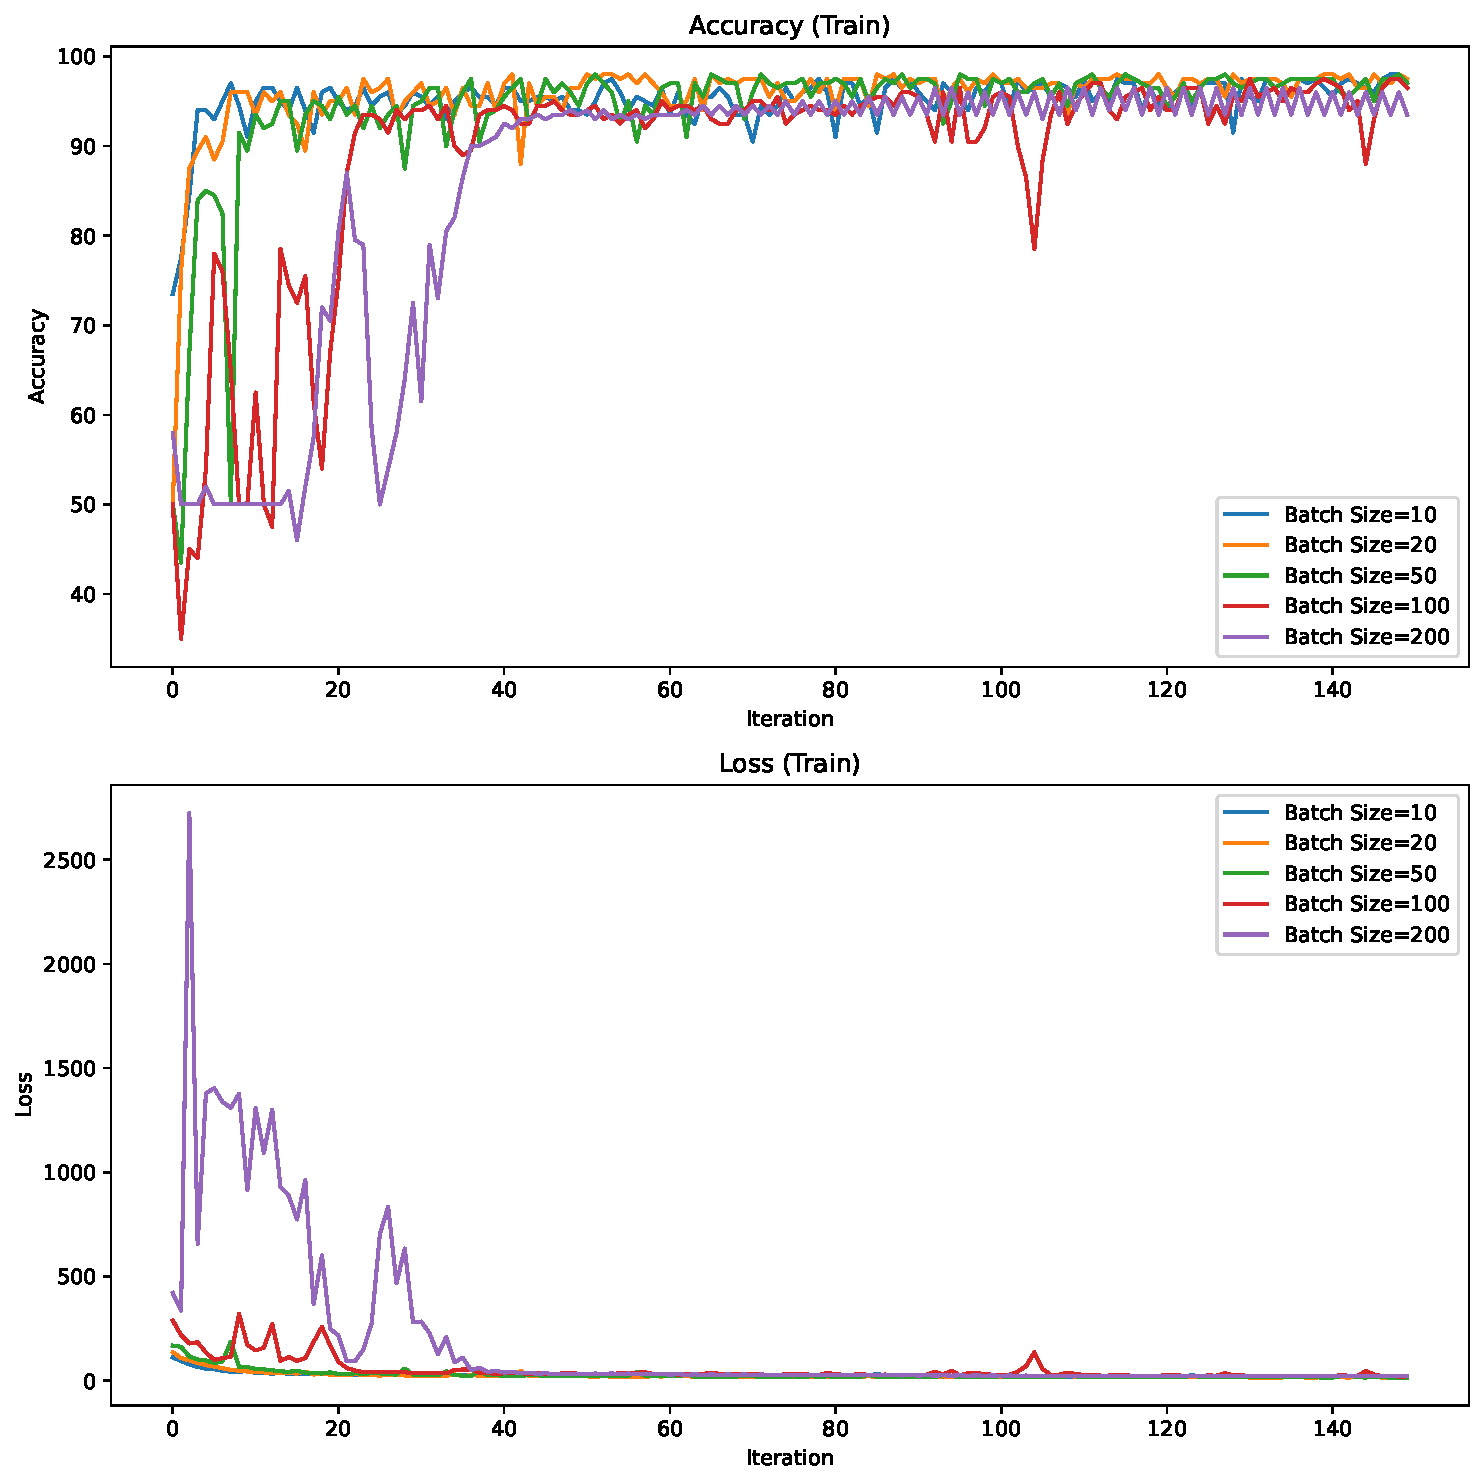
\includegraphics[width=\textwidth]{figs/NN/autograd_batchsize.pdf}
        \caption{Influence of batch size}
        \label{subfig:autograd_batchsize}
    \end{subfigure}
    \begin{subfigure}{0.45\textwidth}
        \centering
        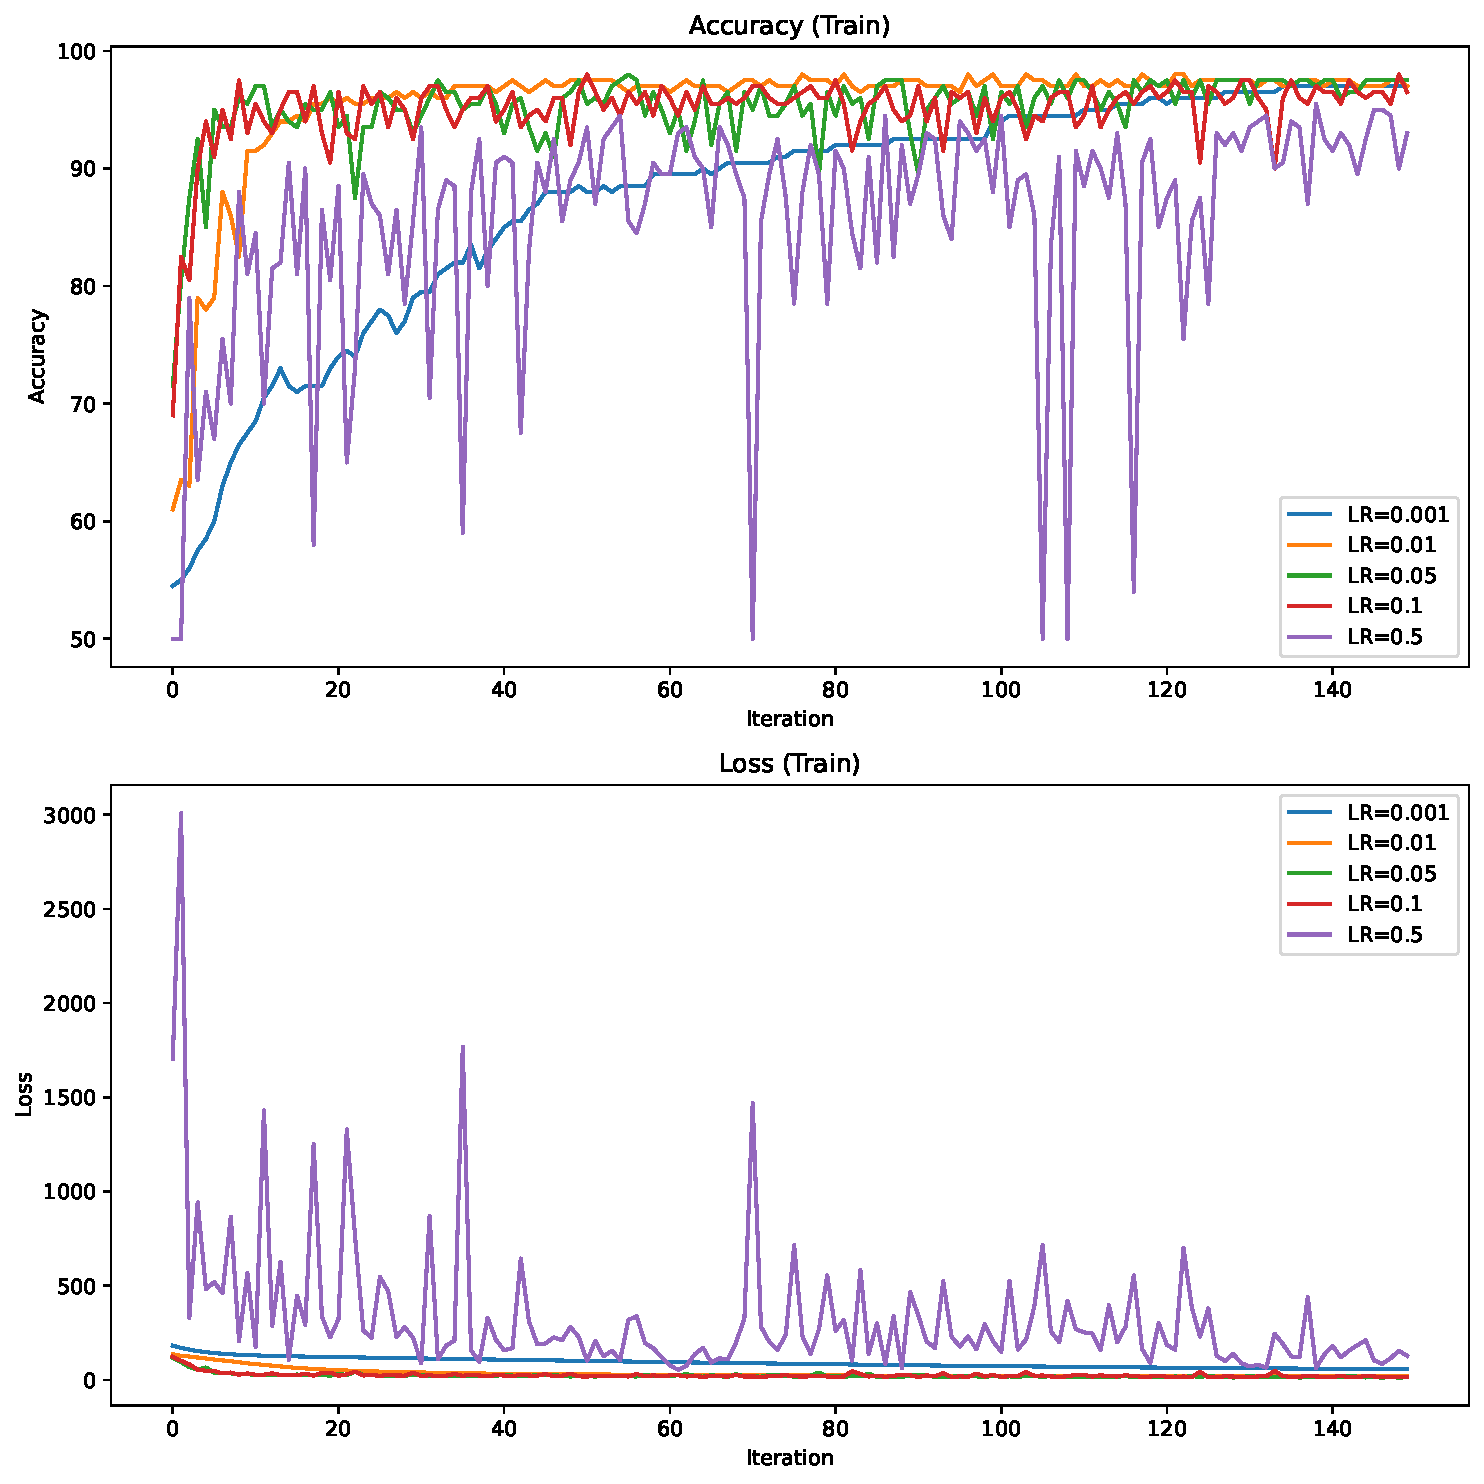
\includegraphics[width=\textwidth]{figs/NN/autograd_lr.pdf}
        \caption{Influence of learning rate}
        \label{subfig:autograd_lr}
    \end{subfigure}
    \caption{Results using \texttt{torch.autograd}}
    \label{fig:autograd}
\end{figure}

\subsection{Simplification of the forward pass with \texttt{torch.nn} layers}

The results of this section can be found in \Cref{fig:torchnn}. In this case, we observe that learning takes longer compared to using manual layers. It requires 150 epochs to reach its maximum performance. This could be attributed to how Torch initializes its layers. However, the training process appears to be more stable, as evidenced by the loss curve.

\begin{figure}[H]
    \centering
    \begin{subfigure}{\textwidth}
        \centering
        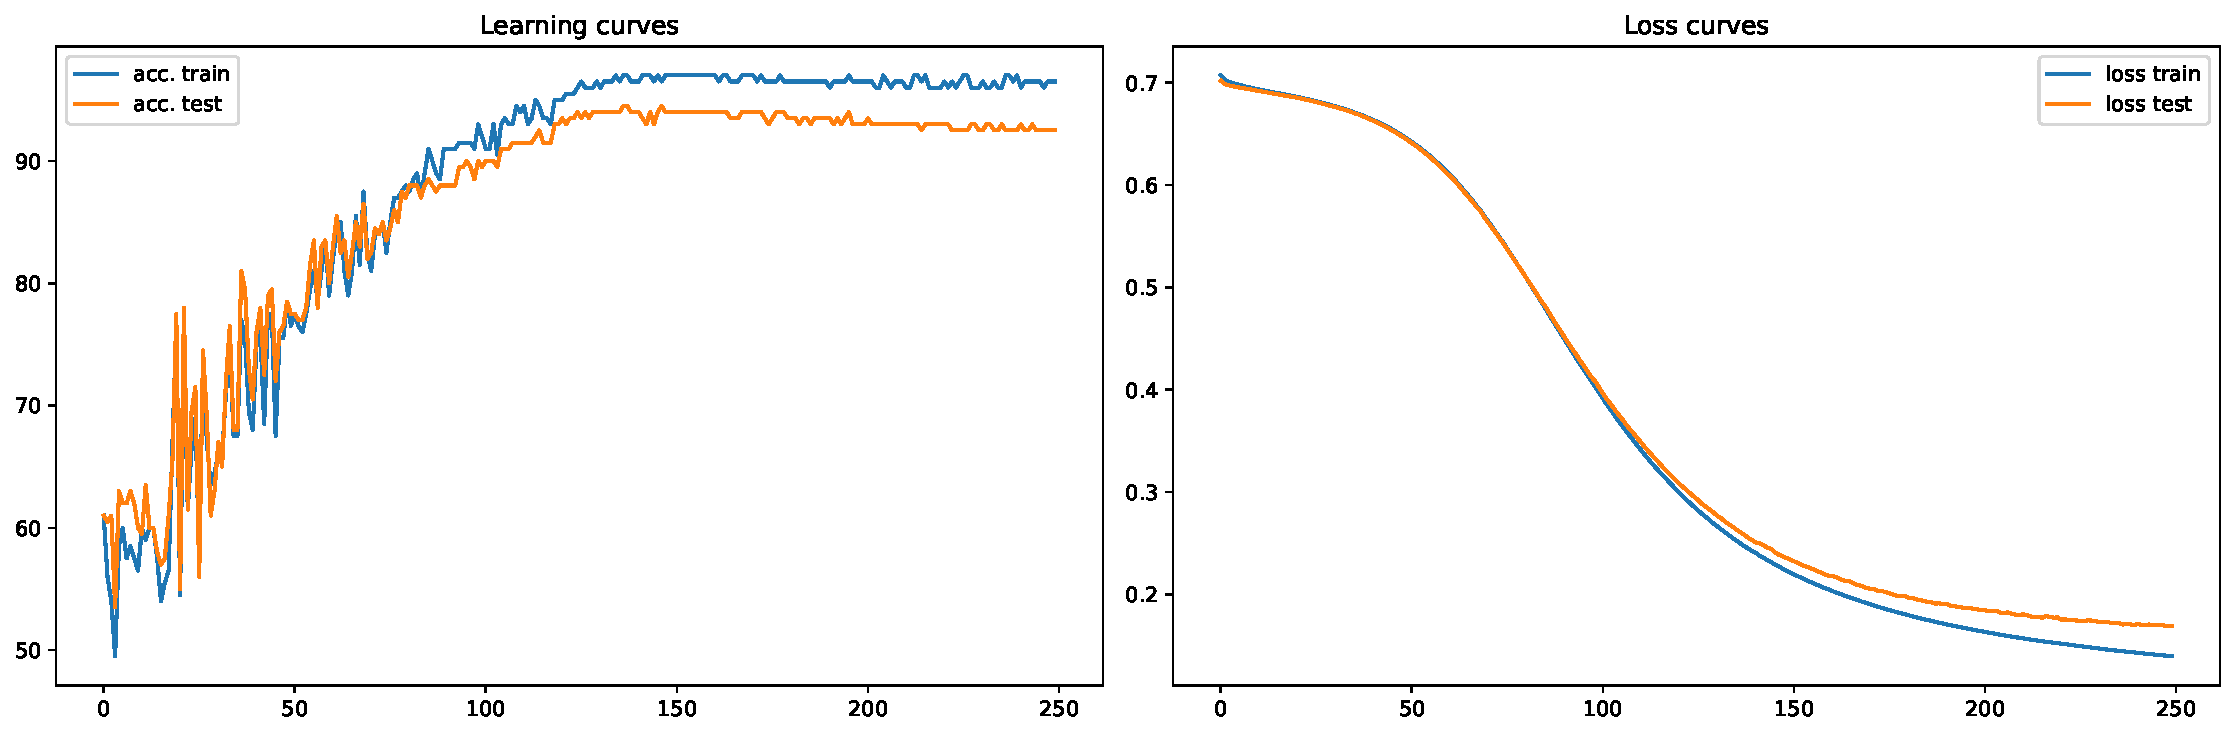
\includegraphics[width=0.88\textwidth]{figs/NN/torchnn_acc_loss.pdf}
        \caption{Accuracy and losses curves using \texttt{torch.nn} layers}
        \label{subfig:torchnn_acc_loss}
    \end{subfigure}
\end{figure}

\begin{figure}[H]\ContinuedFloat
    \centering
    \begin{subfigure}{0.45\textwidth}
        \centering
        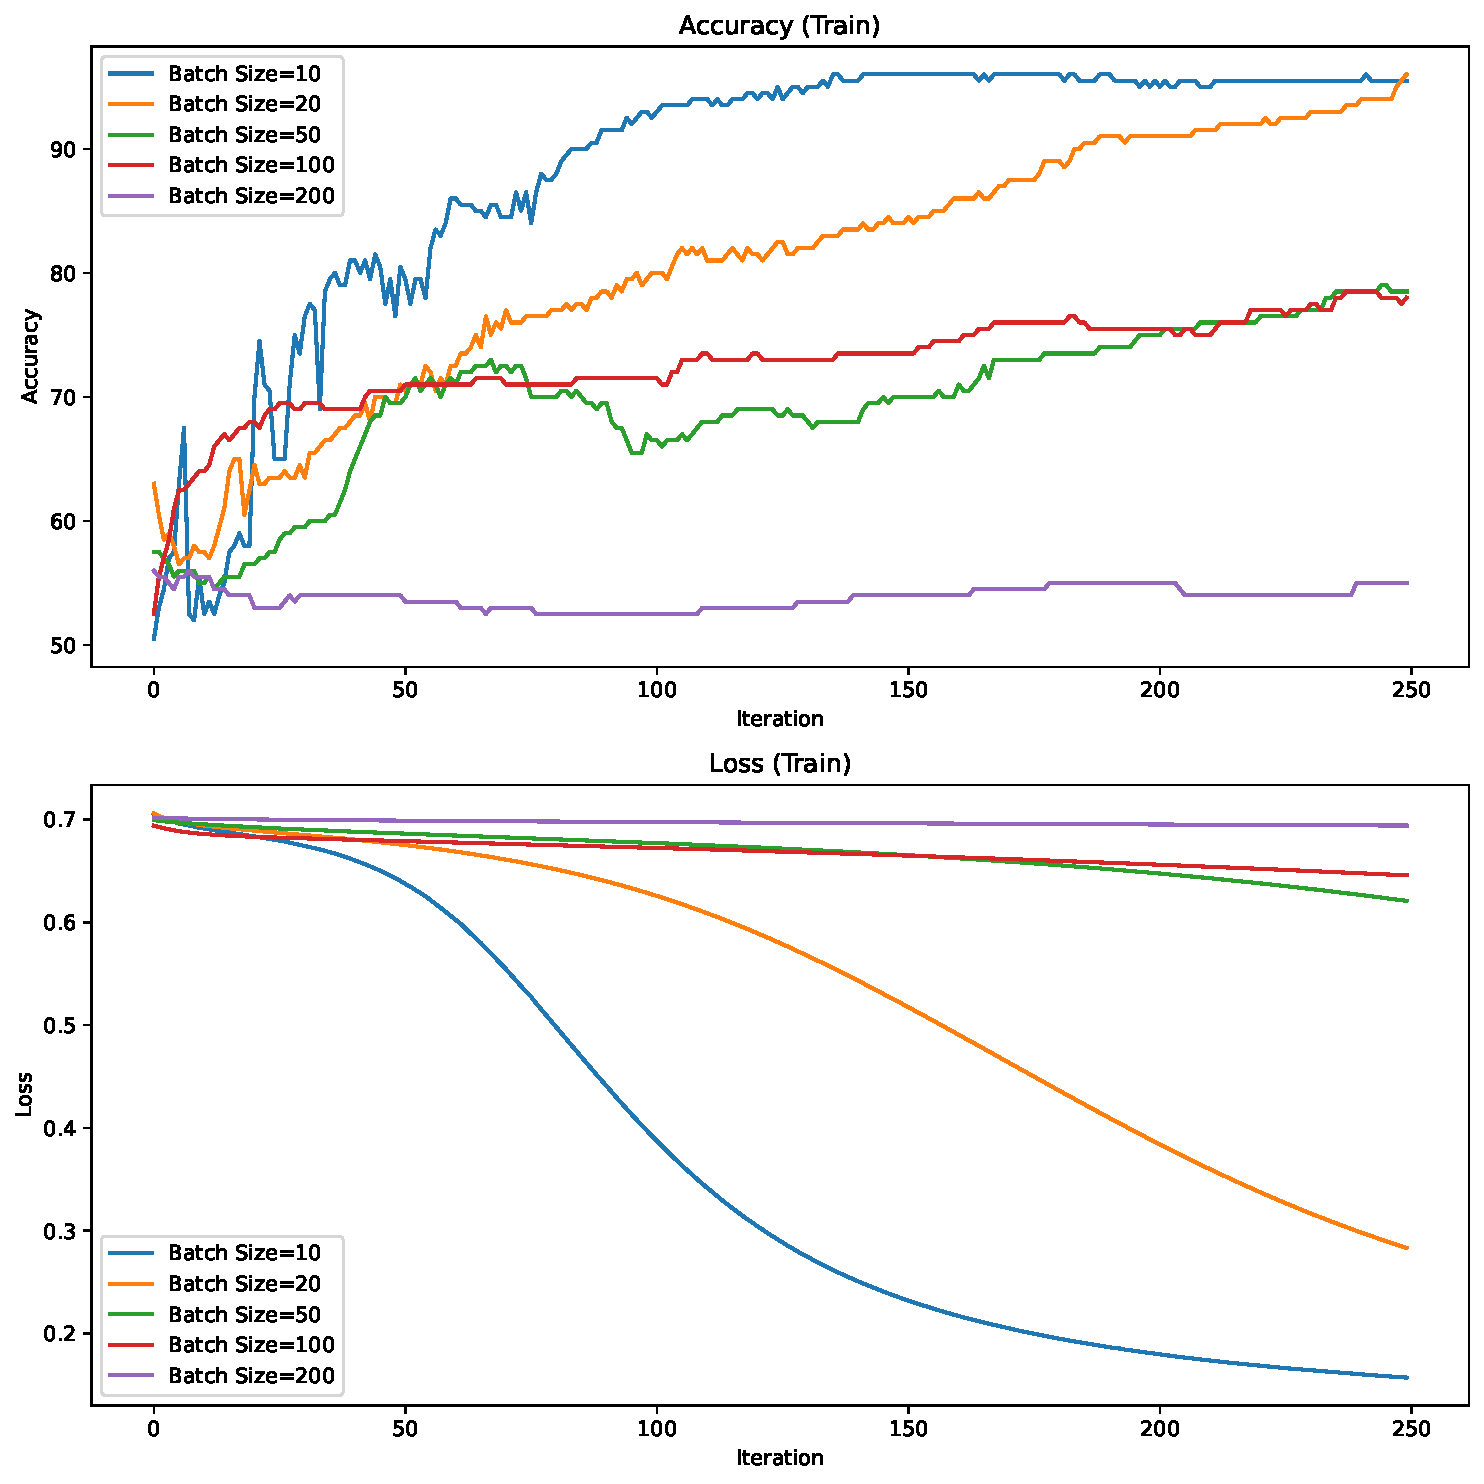
\includegraphics[width=\textwidth]{figs/NN/torchnn_batch_size.pdf}
        \caption{Influence of batch size}
        \label{subfig:torchnn_batchsize}
    \end{subfigure}
    \begin{subfigure}{0.45\textwidth}
        \centering
        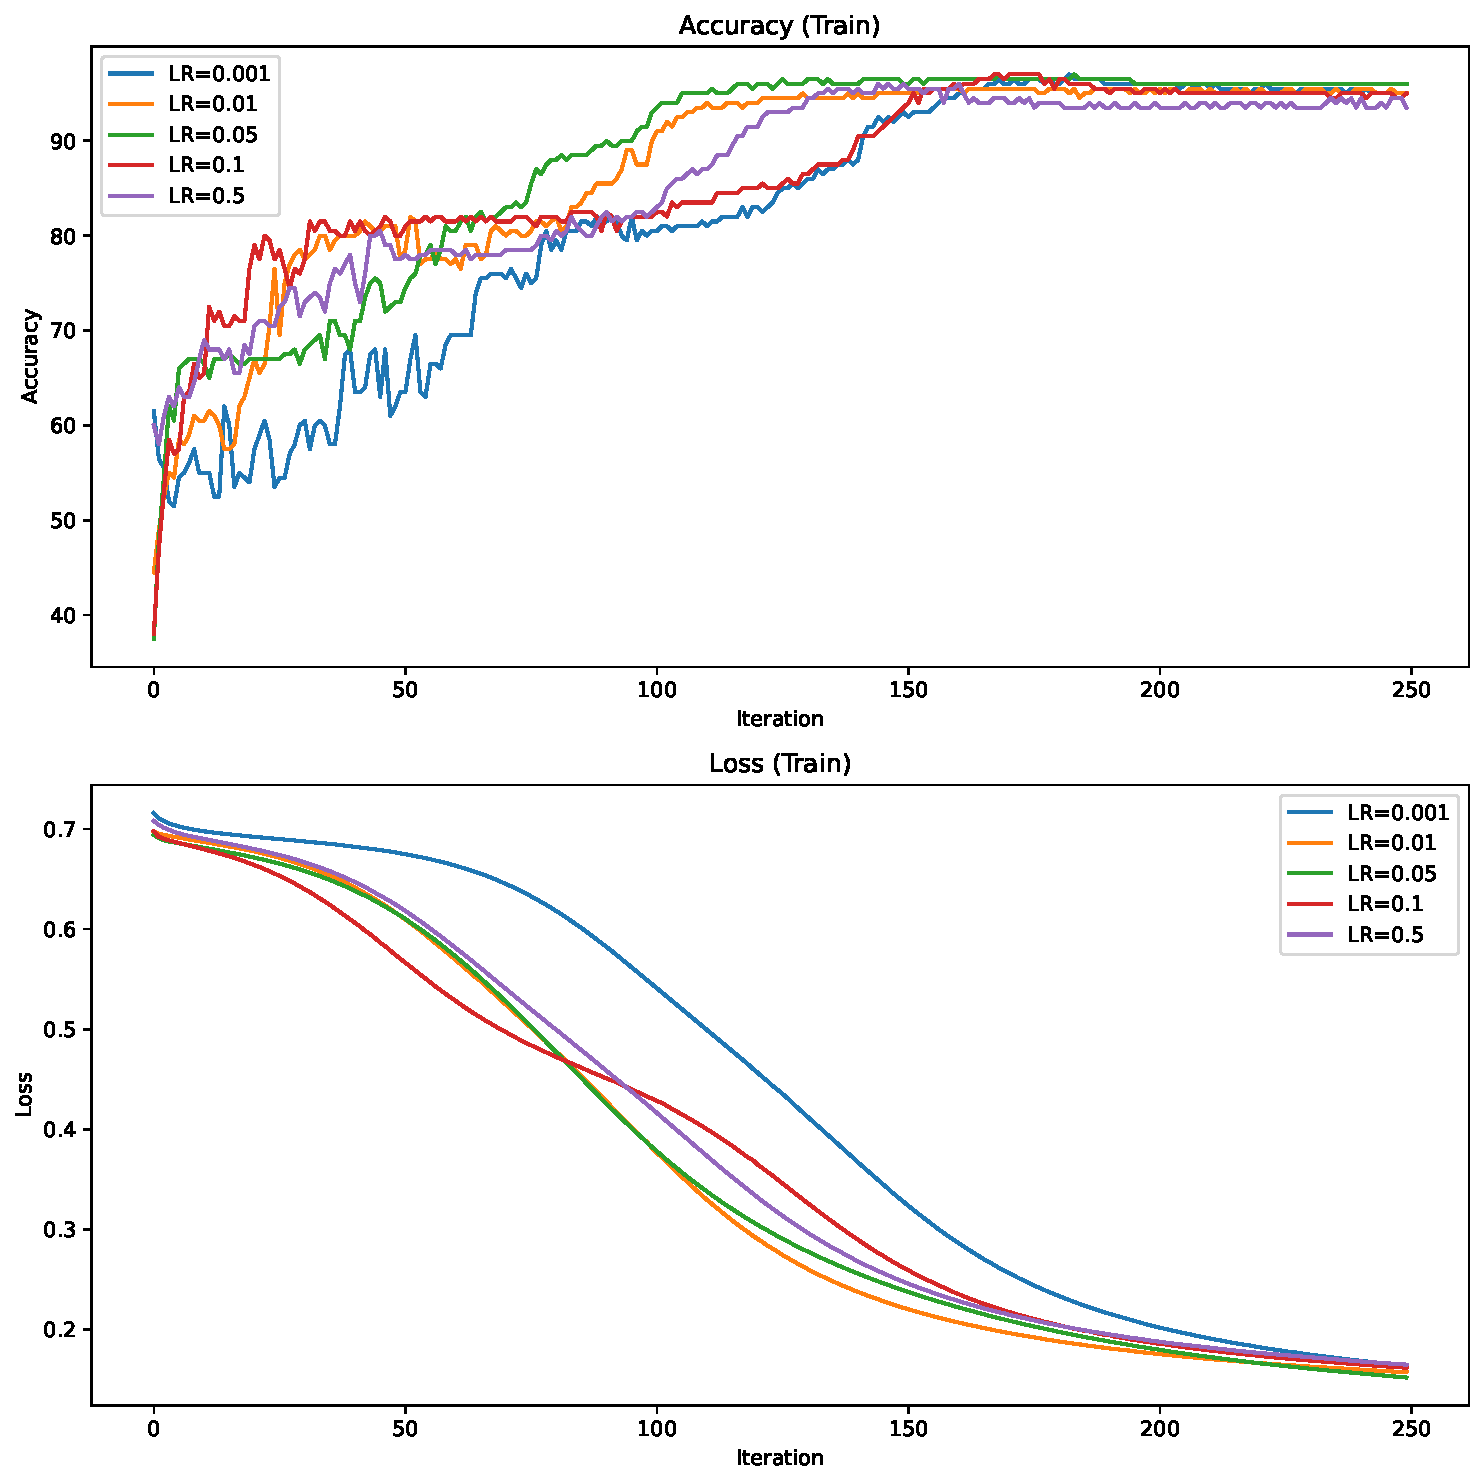
\includegraphics[width=\textwidth]{figs/NN/torchnn_lr.pdf}
        \caption{Influence of learning rate}
        \label{subfig:torchnn_lr}
    \end{subfigure}
    \caption{Results using \texttt{torch.nn}}
    \label{fig:torchnn}
\end{figure}

\subsection{Simplification of the SGD with \texttt{torch.optim}}

The results of this section are presented in \Cref{fig:torchoptim}. The training process is significantly more stable, but it requires a much longer time to converge, taking 300 epochs to reach its maximum performance. 

\begin{figure}[H]
    \centering
    \begin{subfigure}{\textwidth}
        \centering
        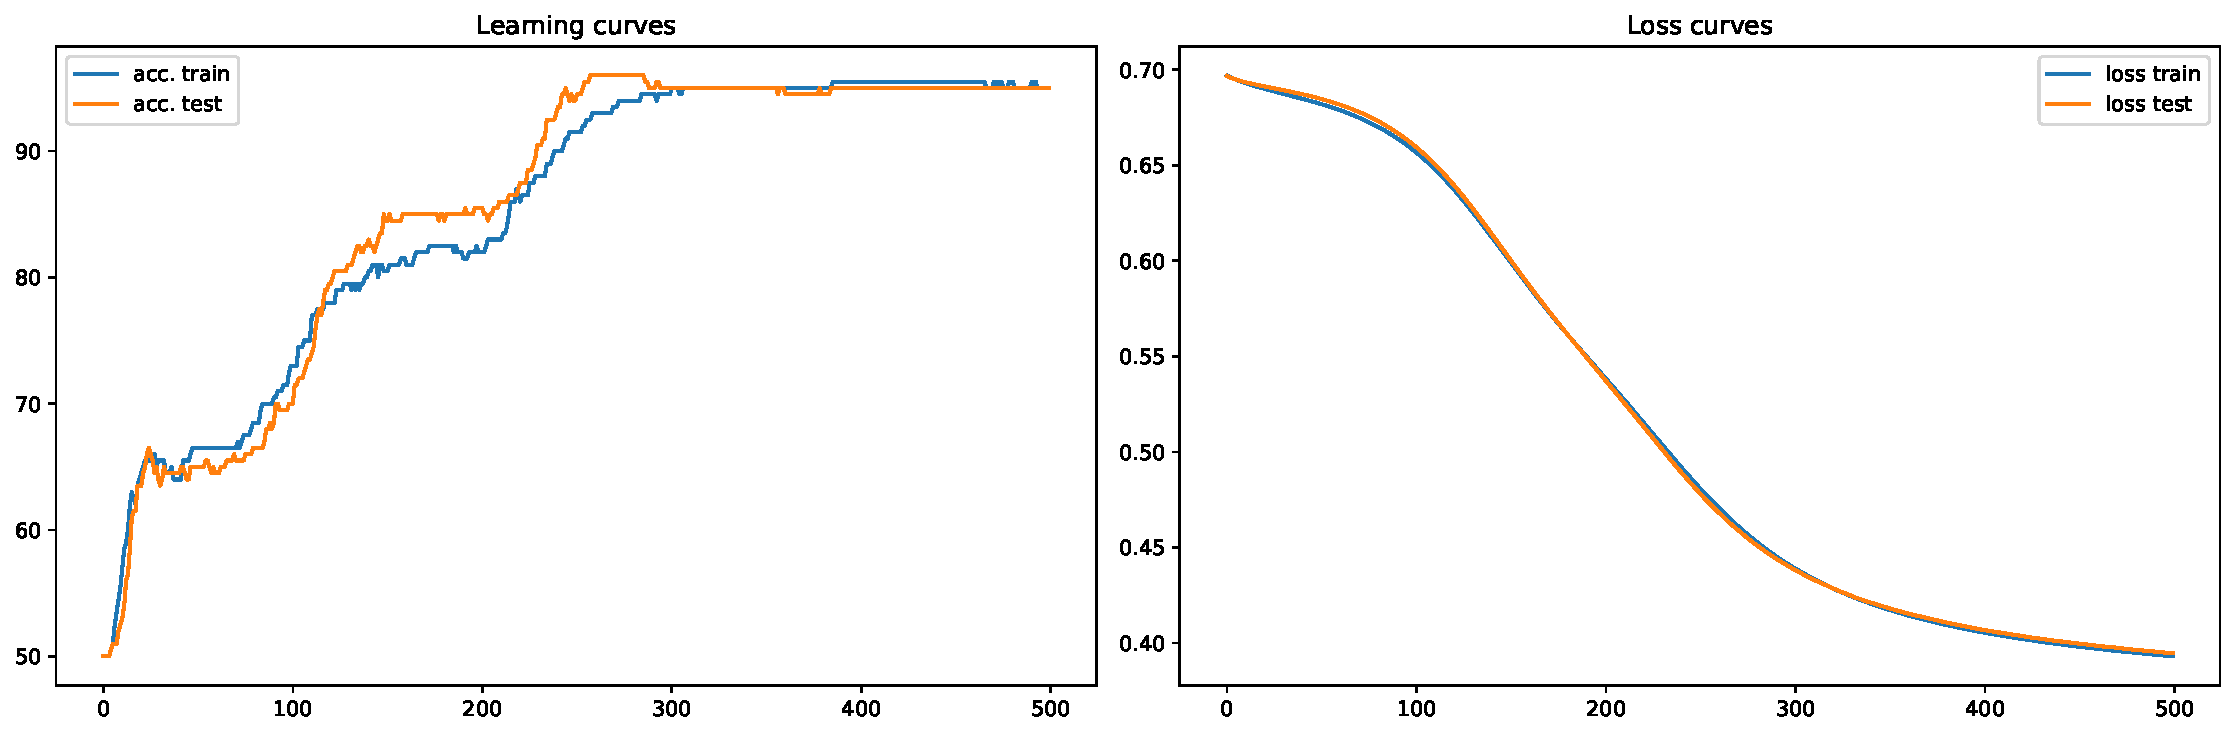
\includegraphics[width=0.88\textwidth]{figs/NN/torchoptim_acc_loss.pdf}
        \caption{Accuracy and losses curves using \texttt{torch.optim}}
        \label{subfig:torchoptim_acc_loss}
    \end{subfigure}
\end{figure}

\begin{figure}[H]\ContinuedFloat
    \centering
    \begin{subfigure}{0.45\textwidth}
        \centering
        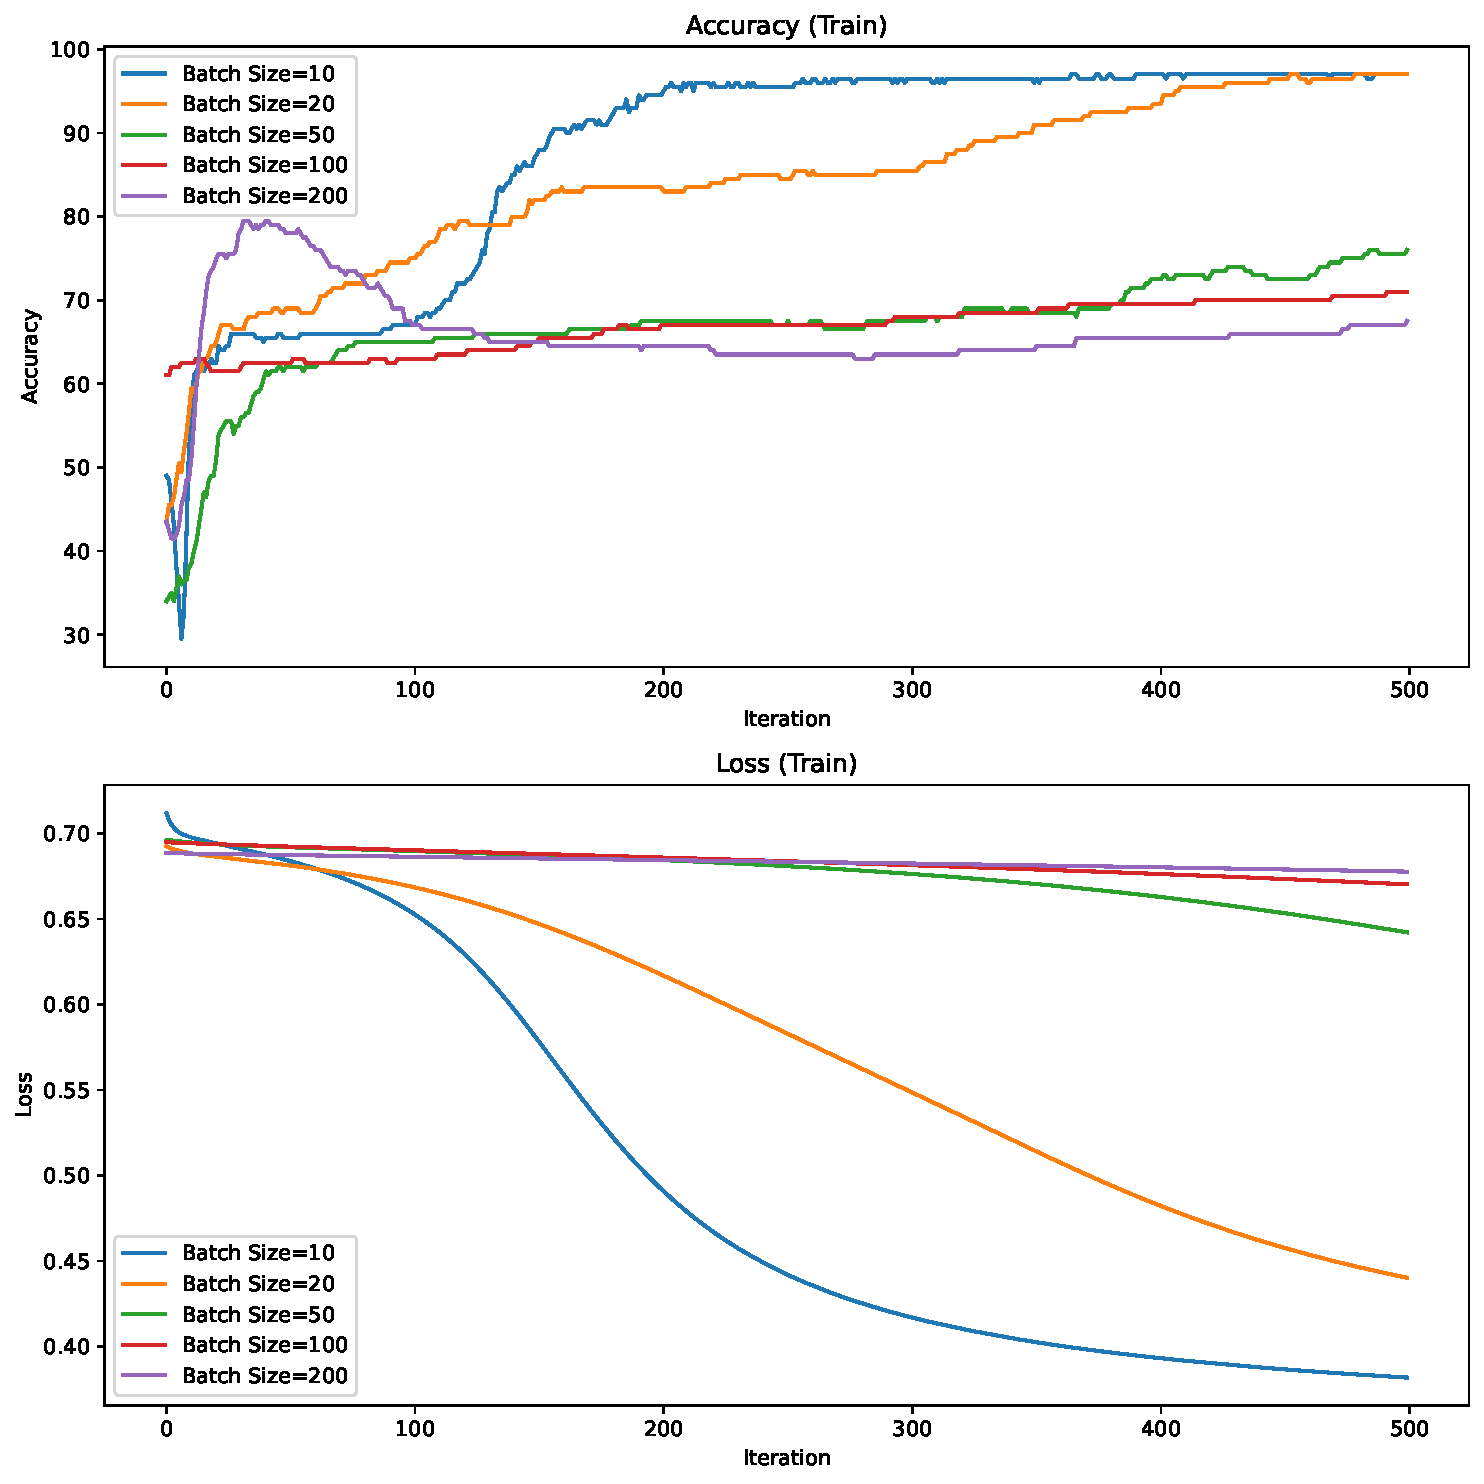
\includegraphics[width=\textwidth]{figs/NN/torchoptim_batchsize.pdf}
        \caption{Influence of batch size}
        \label{subfig:torchoptim_batchsize}
    \end{subfigure}
    \begin{subfigure}{0.45\textwidth}
        \centering
        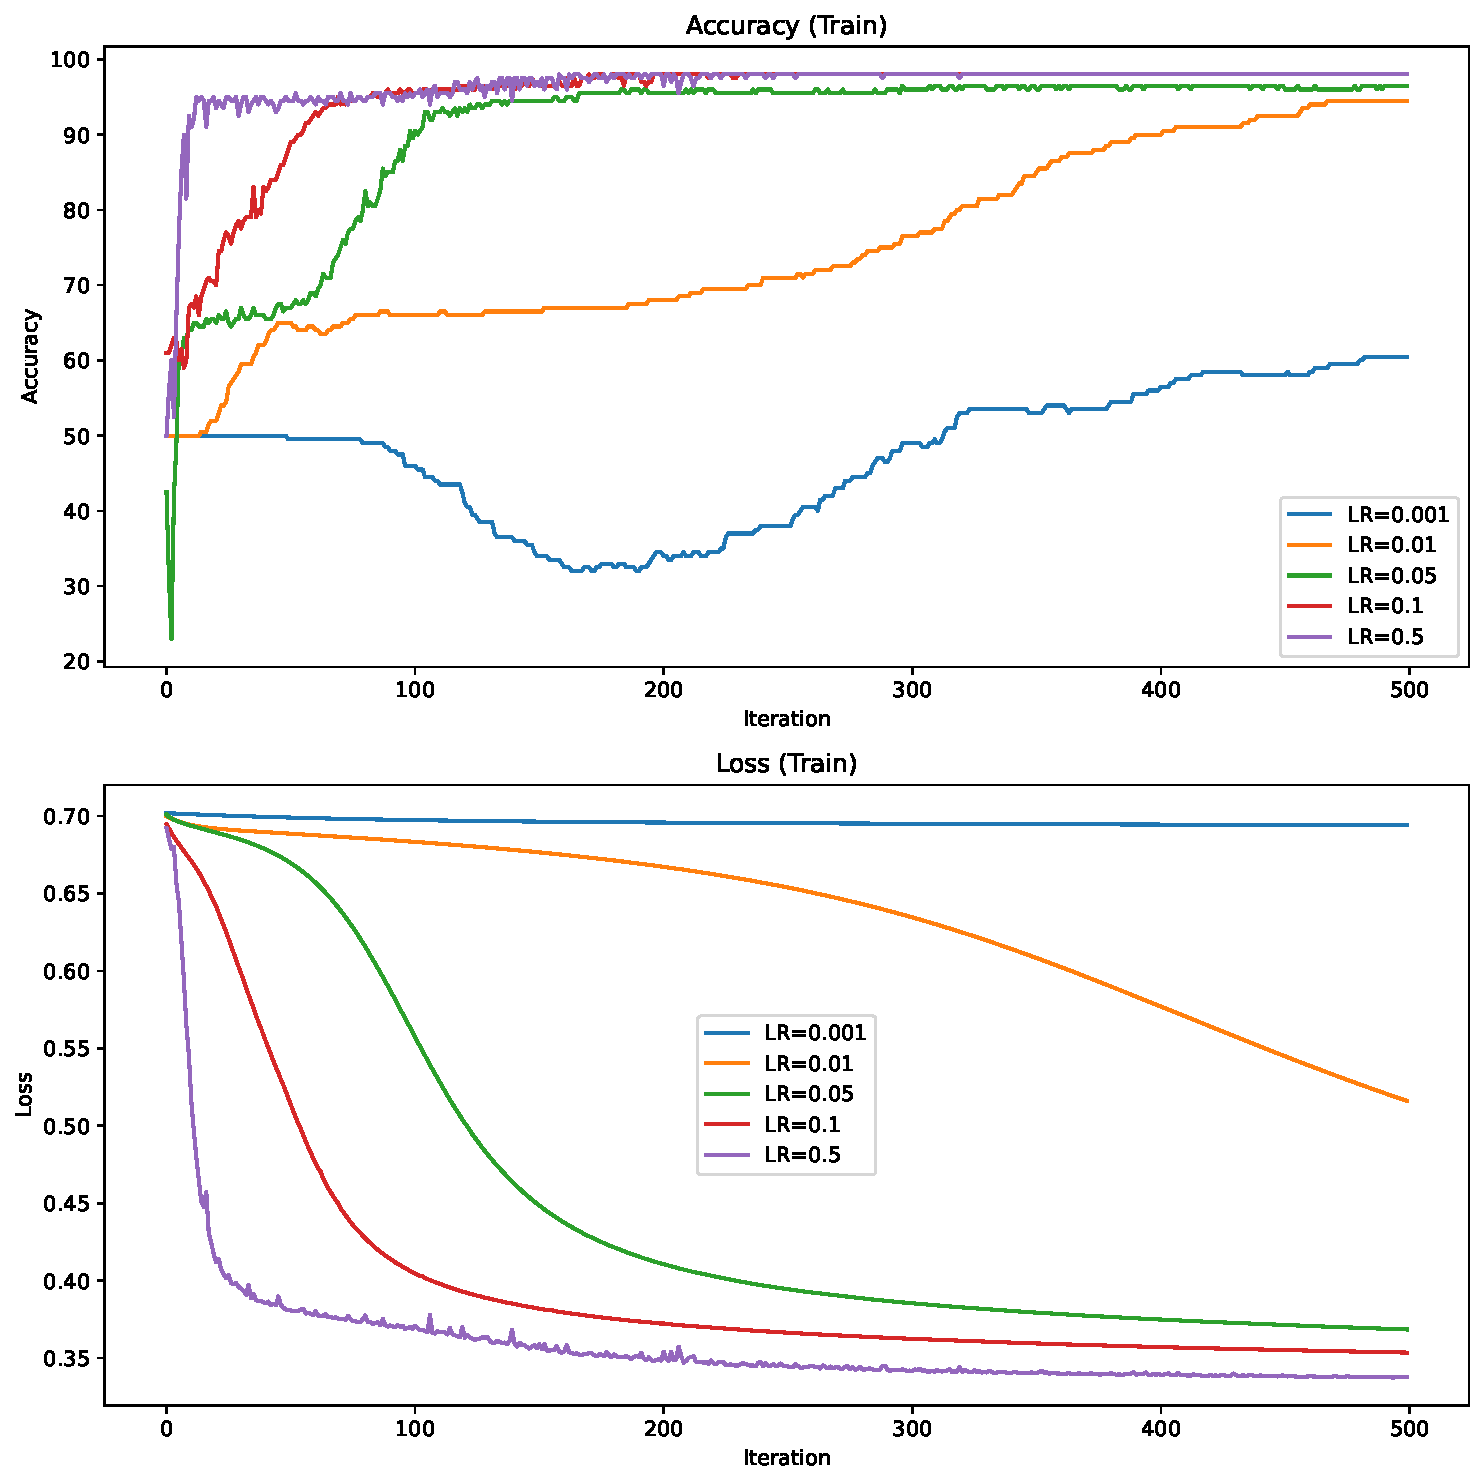
\includegraphics[width=\textwidth]{figs/NN/torchoptim_lr.pdf}
        \caption{Influence of learning rate}
        \label{subfig:torchoptim_lr}
    \end{subfigure}
    \caption{Results using \texttt{torch.optim}}
    \label{fig:torchoptim}
\end{figure}

\subsection{MNIST application}
The following section presents the results of our model on the MNIST dataset, as shown in \Cref{fig:mnist}. Despite its simplicity, the model performs remarkably well. However, there is some instability, which can likely be addressed with a learning rate scheduler or by trying a different optimizer.

\begin{figure}[H]
    \centering
    \begin{subfigure}{\textwidth}
        \centering
        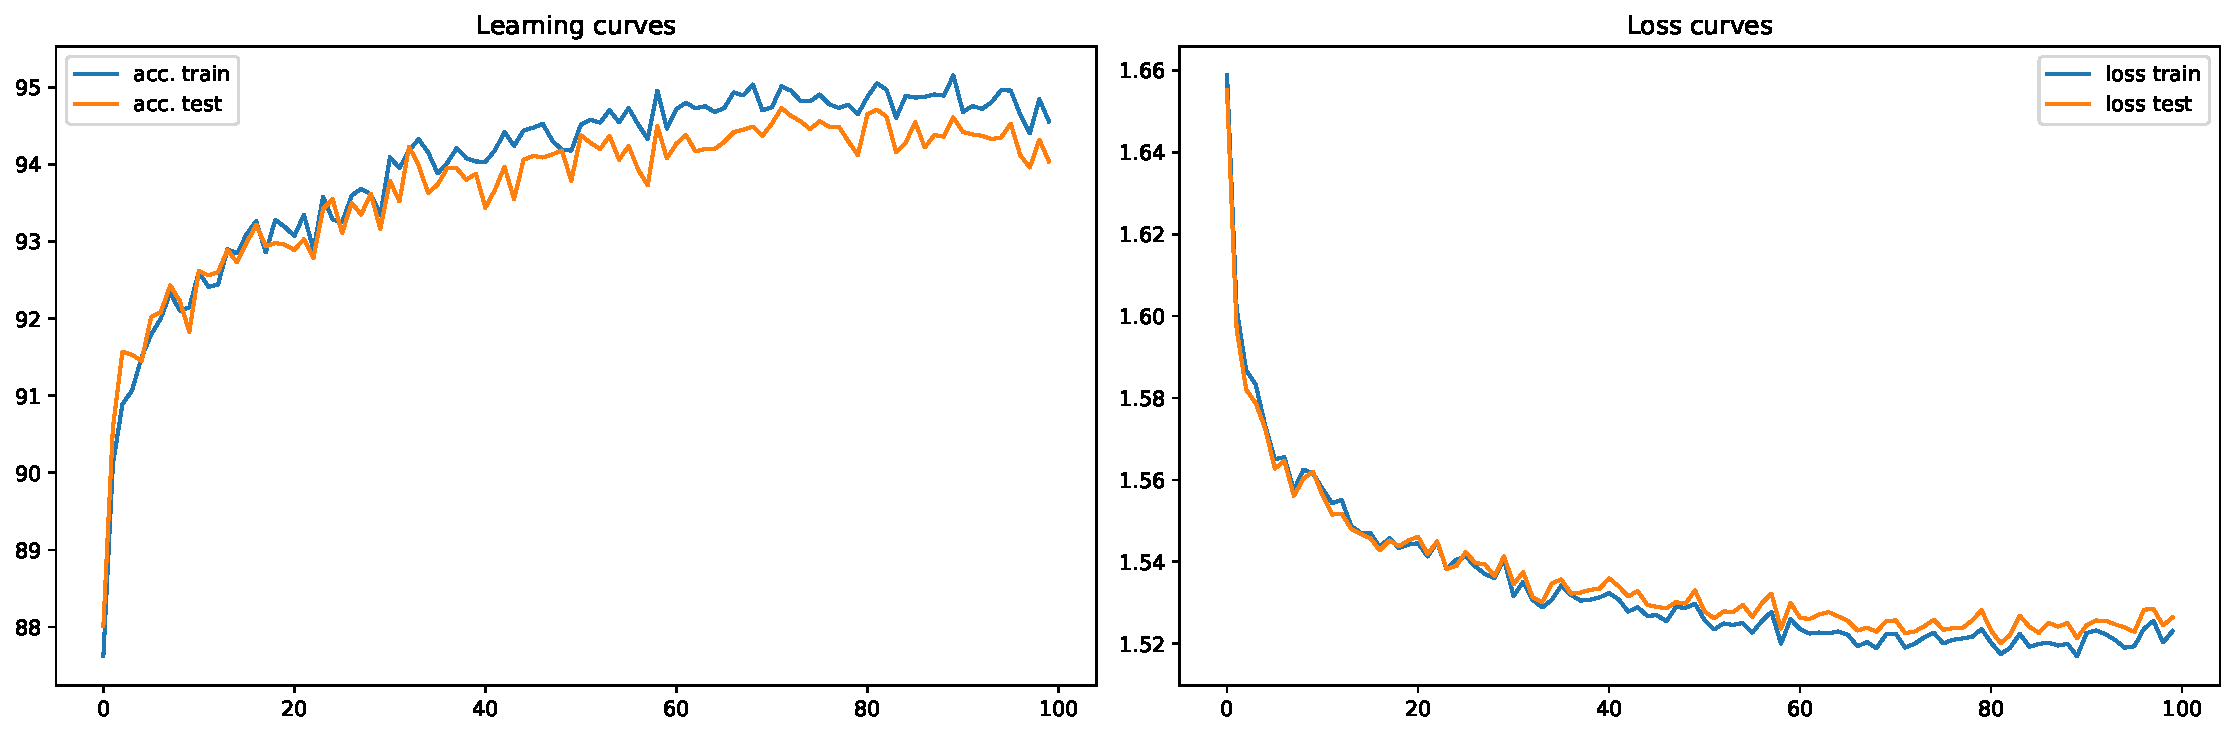
\includegraphics[width=0.88\textwidth]{figs/NN/mnist_acc_loss.pdf}
        \caption{Accuracy and losses curves of our model on MNIST}
        \label{subfig:mnist_acc_loss}
    \end{subfigure}
    \begin{subfigure}{0.45\textwidth}
        \centering
        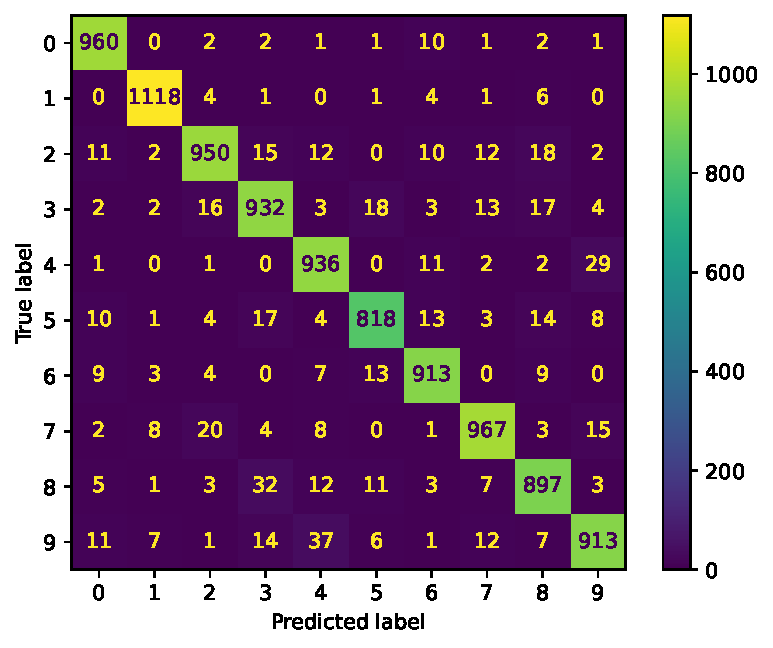
\includegraphics[width=\textwidth]{figs/NN/mnist_cm.pdf}
        \caption{Confusion Matrix}
        \label{subfig:mnist_cm}
    \end{subfigure}
    \caption{Performance on MNIST}
    \label{fig:mnist}
\end{figure}


\subsection{SVM}

We also explored the SVM approach on our circular data, and the decision boundaries, along with their corresponding accuracies, are presented in \Cref{fig:svm_comparison}.

\begin{figure}[H]
    \centering
    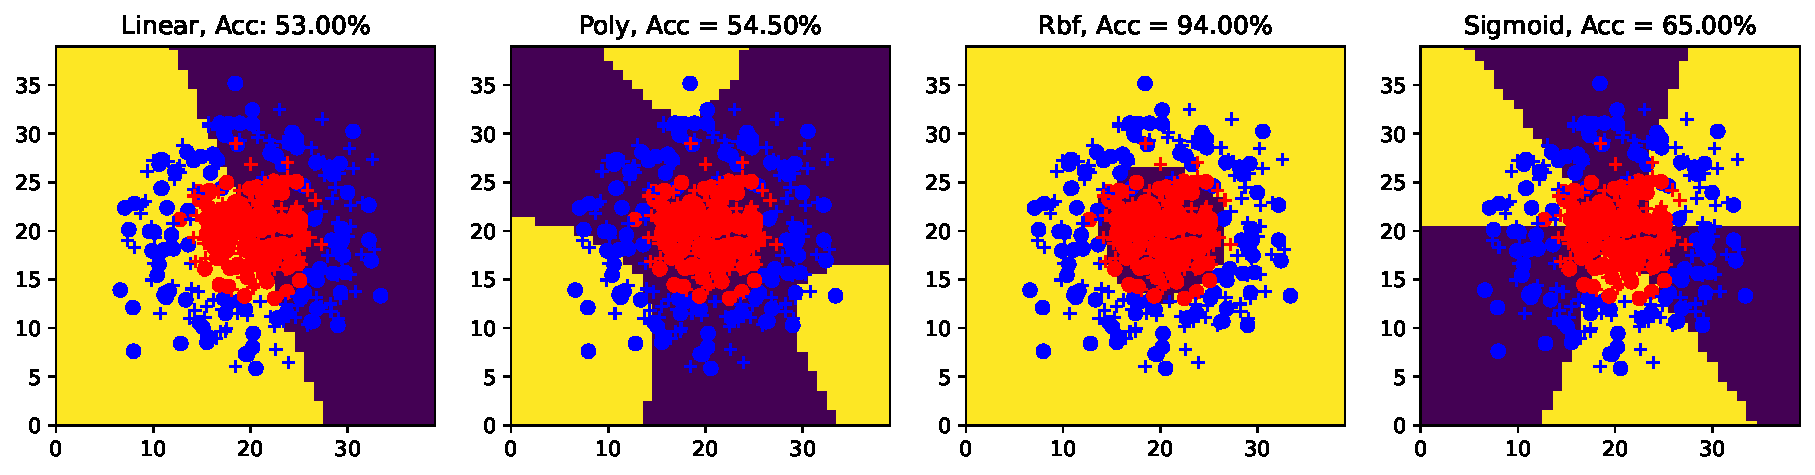
\includegraphics[width=0.9\textwidth]{figs/NN/svm_comparison.pdf}
    \caption{Comparison of SVM}
    \label{fig:svm_comparison}
\end{figure}

It's evident that a linear SVM doesn't work well with circular data. Linear SVMs are designed to find a linear decision boundary that separates data into two classes. Circular data cannot be accurately separated by a single straight line, which is our case here. The Radial Basis Function (RBF) kernel is often the best choice compared to polynomial and sigmoid kernels for circular data because it can capture complex, nonlinear patterns more effectively, and it is better suited to model the circular decision boundaries typically found in such data. RBF kernels can flexibly adapt to various shapes and are more versatile in representing circular patterns, as shown here. It's worth noting that the linear and polynomial kernels did not perform significantly better than a random function.

Furthermore, we conducted experimentations into the influence of the regularization parameter $C$ in the SVM. The results are visualized in \Cref{fig:svm_regularization}. The parameter $C$ in SVMs controls the trade-off between maximizing the margin and minimizing the classification error on the training data. 

When $C$ is large, the SVM aims to minimize the classification error on the training data, which results in a smaller margin, meaning that the decision boundary can be more flexible and may even fit noisy data points. This can lead to overfitting. This effect can especially be seen on the polynomial SVM. 

When $C$ is small, the SVM prioritizes maximizing the margin, even if it means allowing some training points to be misclassified. It results in a larger margin, which often leads to a simpler decision boundary. It encourages the SVM to find a more robust decision boundary that generalizes better to unseen data.

\begin{figure}[H]
    \centering
    \begin{subfigure}{\textwidth}
        \centering
        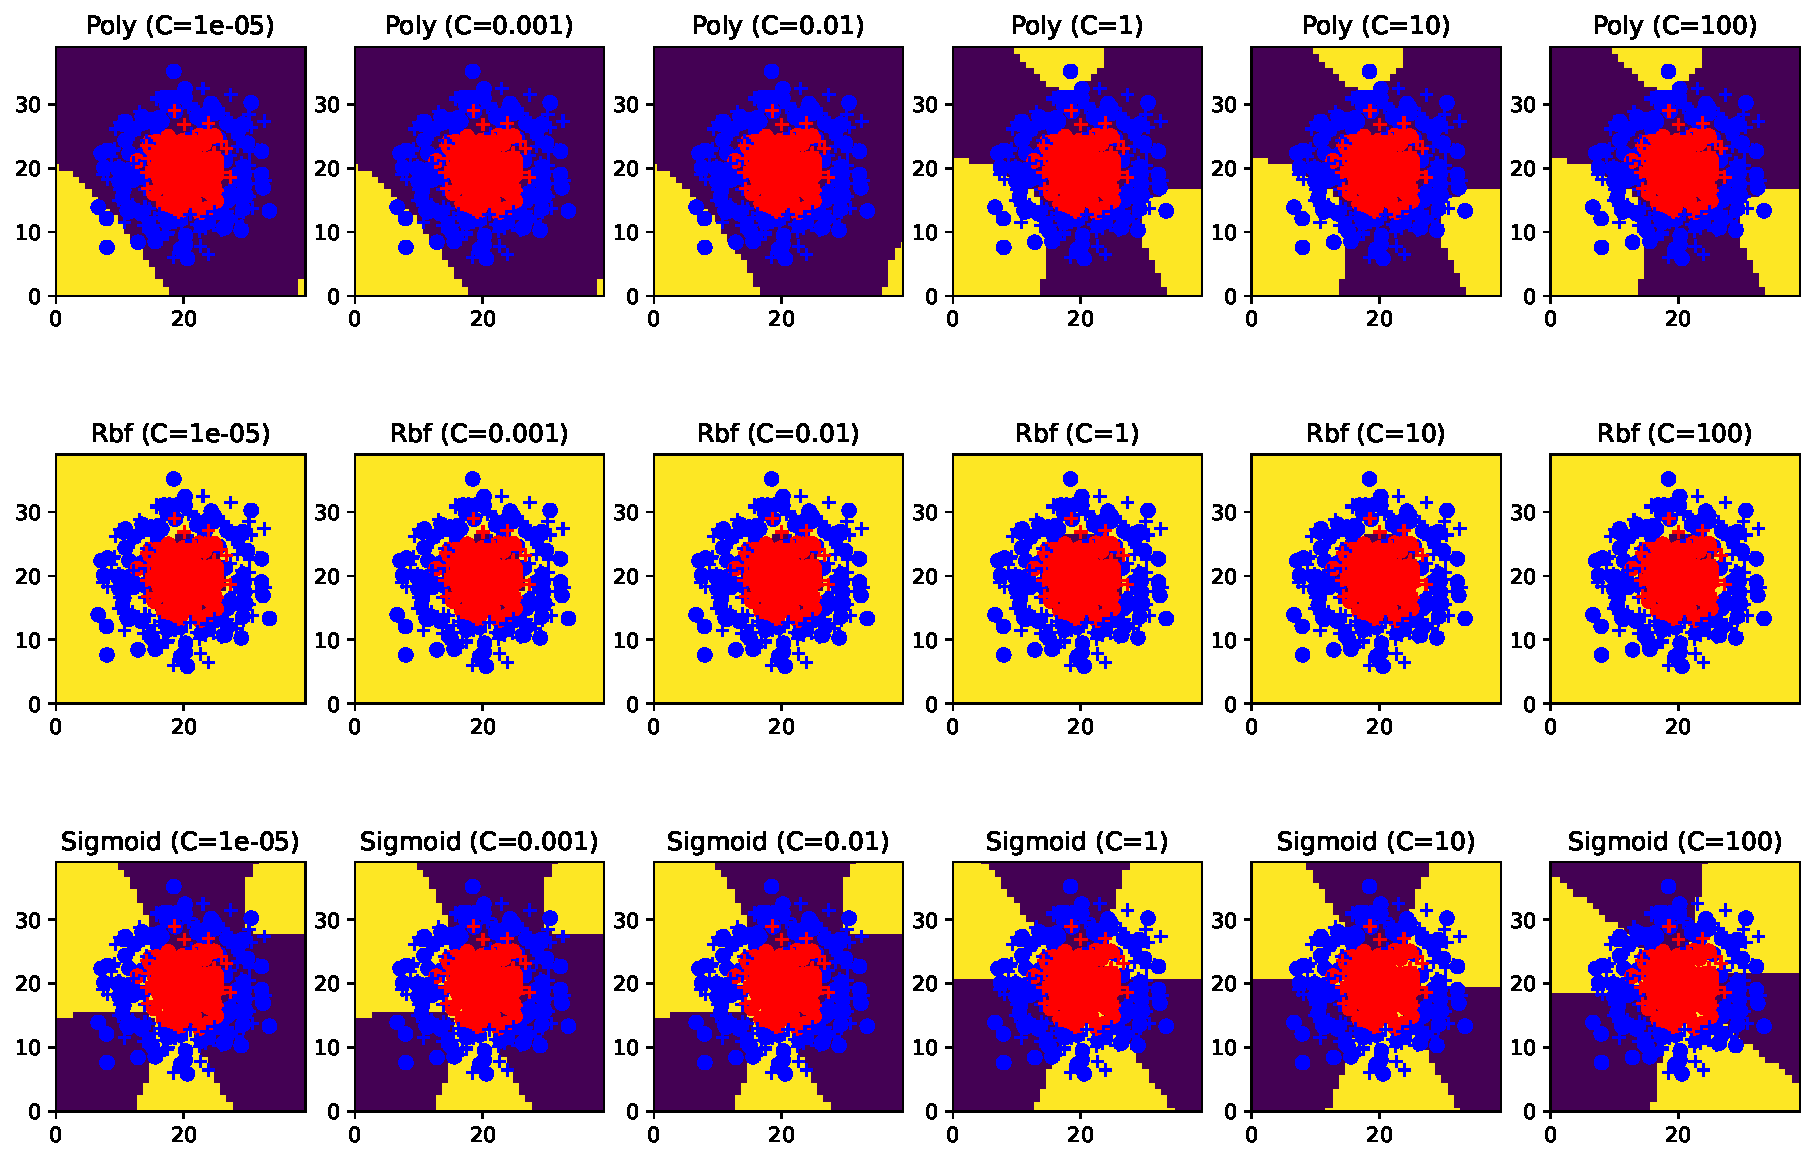
\includegraphics[width=0.9\textwidth]{figs/NN/svm_regularization_grid.pdf}
        \caption{Decision boundaries}
        \label{subfig:svm_regularization_grid}
    \end{subfigure}
\end{figure}

\begin{figure}[H]\ContinuedFloat
    \centering
    \begin{subfigure}{0.9\textwidth}
        \centering
        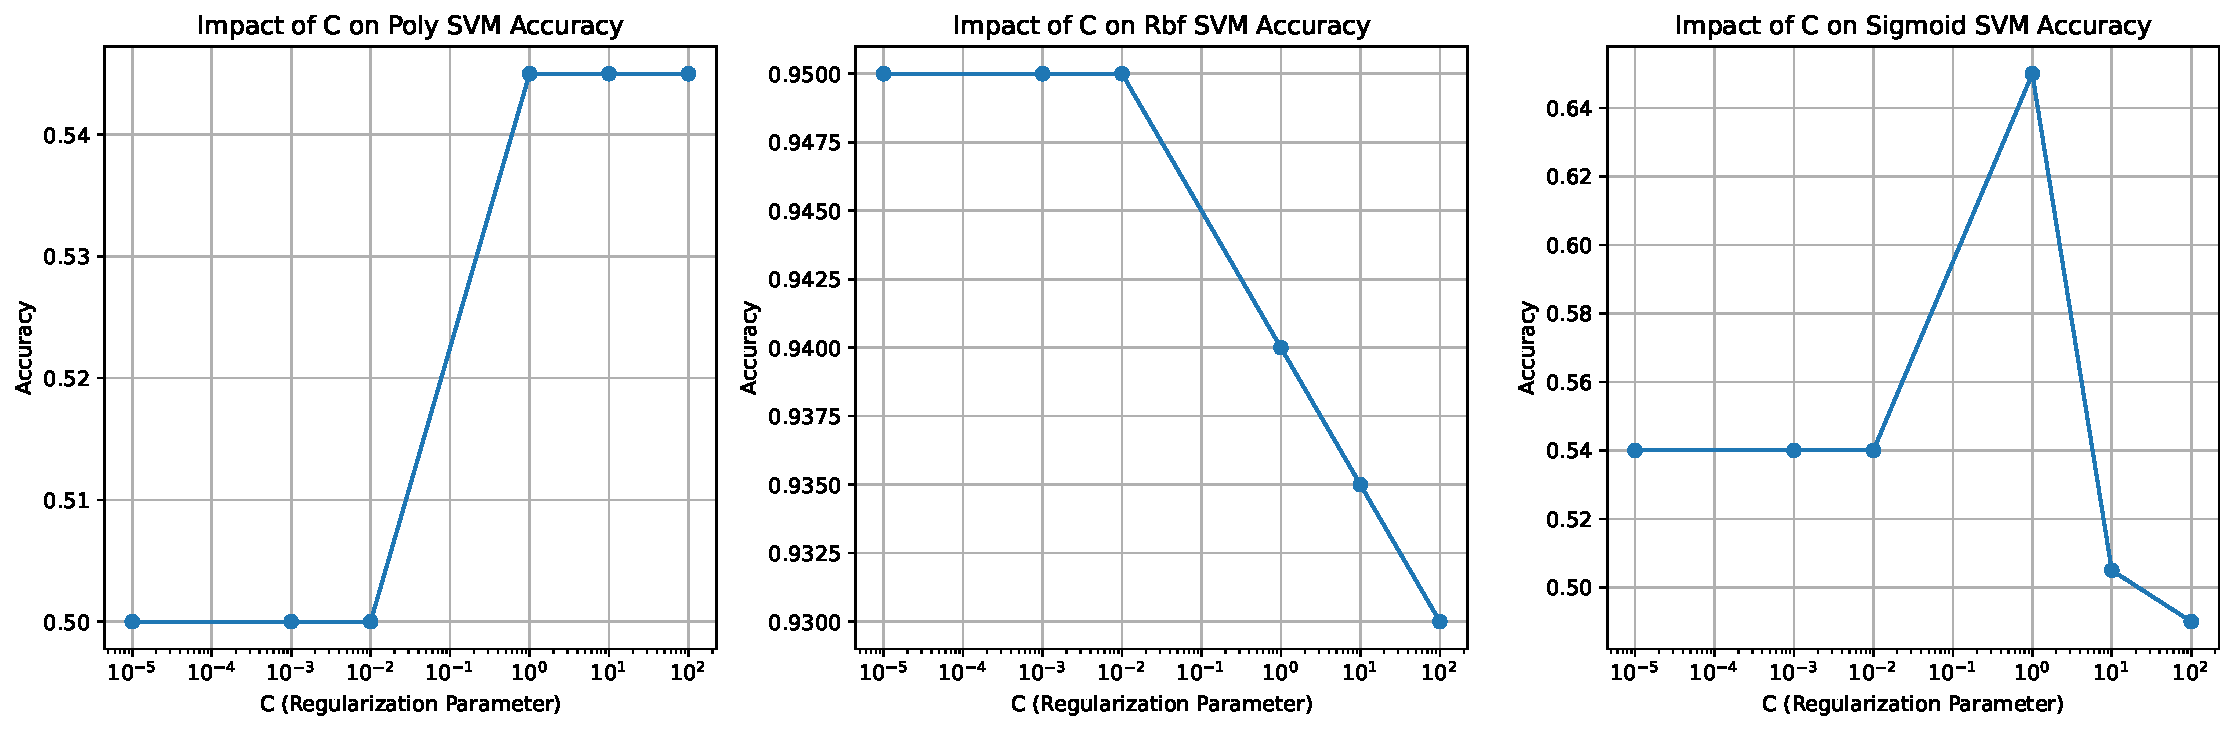
\includegraphics[width=\textwidth]{figs/NN/svm_regularization_acc.pdf}
        \caption{Impact of $C$ on accuracy}
        \label{subfig:svm_regularization_acc}
    \end{subfigure}
    \caption{Influence of regularization parameter}
    \label{fig:svm_regularization}
\end{figure}
